\documentclass[12pt, a4paper, twoside, openright]{book}

\usepackage{fontspec}
\setmainfont{texgyrepagella}[
  Extension = .otf,
  UprightFont = *-regular,
  BoldFont = *-bold,
  ItalicFont = *-italic,
  BoldItalicFont = *-bolditalic,
]
\newfontfamily{\Symbola}{[Symbola.ttf]}

\usepackage{thesis/vuwthesis} % sets up some local things, mostly the front page

\usepackage{url} % for typesetting urls
\usepackage{amsfonts}
\usepackage{amsmath}
\usepackage{biblatex}
\addbibresource{myrefs.bib}

\usepackage{unicode-math}

\usepackage{amsthm}



\DeclareMathAlphabet{\mathcal}{OMS}{cmsy}{m}{n}
\let\mathbb\relax % remove the definition by unicode-math
\DeclareMathAlphabet{\mathbb}{U}{msb}{m}{n}


\usepackage[dvipsnames]{xcolor}
\newcommand\myshade{85}
\usepackage{todonotes}
\setuptodonotes{inline}

\colorlet{mylinkcolor}{Black}
\colorlet{mycitecolor}{YellowOrange}
\colorlet{myurlcolor}{NavyBlue}

\usepackage[colorlinks]{hyperref}
\hypersetup{
    pdftitle={Maxwell Clarke MSc Proposal},
    pdfsubject={Conditional Generative Transformers for Hand-Guided Animation Automation},
    pdfauthor={Maxwell Clarke},
    pdfkeywords={Artificial Intelligence, AI, Machine Learning, ML, Neural Networks, Deep Learning, Transformers, Transformer models, Gaussian Processes, Bayesian Inference, Animation, Virtual Reality, VR, Skeletal Animation, Character Animation, Victoria University of Wellington, VUW},
    linkcolor  = mylinkcolor!\myshade!black,
    citecolor  = mycitecolor!\myshade!black,
    urlcolor   = myurlcolor!\myshade!black,
    colorlinks = true,
}

\usepackage[nameinlink]{cleveref}

%\renewcommand{\baselinestretch}{1.00}

\newcommand{\R}{\mathbb{R}}
\newcommand{\N}{\mathbb{N}}
\newcommand{\E}{\mathsf{E} }
\newcommand{\x}{\mathbfit{x}}
\newcommand{\X}{\mathbfit{X}}
\newcommand{\vb}{\mathbfit{b}}
\newcommand{\erf}{\operatorname{erf}}
\newcommand{\relu}{\phi_{\text{relu}}}
\newcommand{\gelu}{\phi_{\text{gelu}}}

\newcommand{\TODO}[1]{\todo{todo: #1}}

\DeclareMathOperator{\attn}{attn}

% with alignment
\newcommand{\fdef}[3]{#1 &\colon #2 \to #3}
\newcommand{\vfdef}[3]{\fdef{#1}{\R^{#2}}{\R^{#3}}}
% [n]o alignment
\newcommand{\nfdef}[3]{#1 \colon #2 \to #3}
\newcommand{\nvfdef}[3]{\nfdef{#1}{\R^{#2}}{\R^{#3}}}


\begin{document}

\frontmatter
% Book style knows about front matter
% Report style doesn't so you need to set roman numbering etc yourself :-(

%%%%%%%%%%%%%%%%%%%%%%%%%%%%%%%%%%%%%%%%%%%%%%%%%%%%%%%

\title{Conditional Generative Transformers for Hand-Guided Animation Automation}
\author{Maxwell Clarke}

\subject{Computer Science}
\abstract{
In this thesis I develop neural networks and apply them to the problem of hand motion modelling for film production.

Firstly, I develop a novel training regime for transformers which allows auto-regressive sampling of high-dimensional data in an arbitrary order, and demonstrate this technique on pixel-by-pixel sampling of MNIST images.

Secondly, I develop a predictive model for hand-motion data, via unsupervised training on a motion-capture dataset. I compare fixed-order sampling to best order I found using the above technique.
}
% Books don't normally have abstracts, and this is a bit of a hack

% Uncomment the appropriate degree
%\phd
% \mscthesisonly
%\mscwithhonours
\mscbothparts
% \otherdegree{DEGREE OR DIPLOMA NAME}



%%%%%%%%%%%%%%%%%%%%%%%%%%%%%%%%%%%%%%%%%%%%%%%%%%%%%%%




\maketitle

\include{thesis/thesis-acknowledge}

\tableofcontents


%%%%%%%%%%%%%%%%%%%%%%%%%%%%%%%%%%%%%%%%%%%%%%%%%%%%%%%

% book style knows about mainmatter
% if you are using report style you will have to rest page numbering etc.
\mainmatter


%%%%%%%%%%%%%%%%%%%%%%%%%%%%%%%%%%%%%%%%%%%%%%%%%%%%%%%

% individual chapters included here


%!!!!!!!!!!!!!!!!!!!!!!!!!!!!!!!!!!!!!!!!!
% Credit for the hand mesh
% "Robotic Hand" (https://skfb.ly/6XLBS) by SeanNicolas is licensed under Creative Commons Attribution (http://creativecommons.org/licenses/by/4.0/).
%!!!!!!!!!!!!!!!!!!!!!!!!!!!!!!!!!!!!!!!!!


\chapter{Introduction}
\label{C:intro}

\begin{figure}[t]
\centering
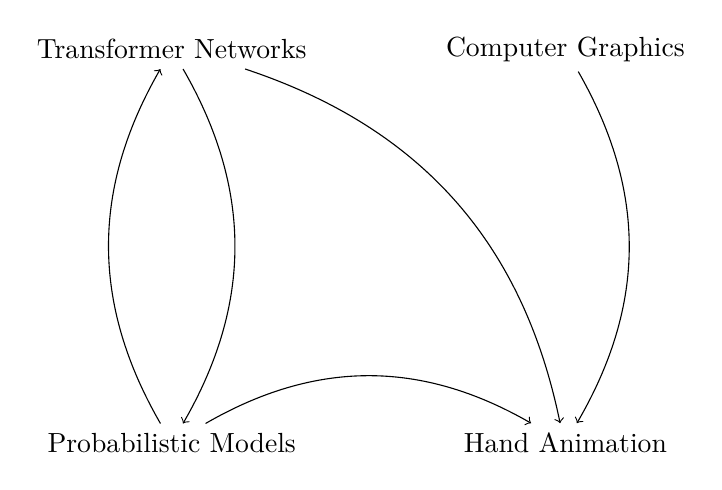
\begin{tikzpicture}
    \tikzstyle{every node}=[node distance=5cm]
    \node (tn) {Transformer Networks};
    \node (pm) [below of=tn] {Probabilistic Models};
    \node (cg) [right of=tn] {Computer Graphics};
    \node (an) [below of=cg] {Hand Animation};

    \draw[->,bend left] (tn) to (pm);
    \draw[->,bend left] (pm) to (tn);
    \draw[->,bend left] (cg) to (an);
    \draw[->,bend left] (pm) to (an);
    \draw[->,bend left] (tn) to (an);
\end{tikzpicture}
\caption[The relationship between the different fields in this thesis]{How learnings and experiments from different fields contribute to each other in this thesis.}
\end{figure}

This thesis introduces concepts and experiments at the intersection of two areas: Deep Learning and Computer Graphics. There are three main areas of focus: Comprehensively introducing a class of neural network models called \textit{transformer} networks; an experiment comparing different sampling orders when predicting data using\textit{auto-regressive} transformer models; and the developement of an application of auto-regressive transformer models for \textit{hand pose modeling}.

\section{Contributions}

Although much of the work done is summarizing others' research and presenting learnings, there are two main novel contributions:
\begin{enumerate}
    \item I present experiments with \textit{dynamically-ordered} auto-regressive sampling, utilising the \textit{permutation-invariance} property of the attention operation in transformer models.
    \item I present a proof-of-concept transformer-based generative model for hand motion prediction, which can be used to predict hand motion at arbitrary target frames, and to predict the joints of a hand in any order within that frame.
\end{enumerate}
These contributions involved training neural networks (see \Cref{fig:context}), in particular transformers, on two datasets - MNIST, and a motion capture dataset of hand motion. The results of these experiments are presented in \Cref{C:a-o-sampling} and \Cref{C:hand-model} respectively.

\begin{figure}
    \centering
    
\pgfdeclarelayer{bg}
\pgfsetlayers{bg,main}

\begin{tikzpicture}
    \tikzstyle{every node}=[node distance=3.5cm,minimum height=0.8cm]

    % dataset type
    \node (datasettype) {Dataset Type};
    \node[draw, below of=datasettype] (seqpred) {Sequence Prediction};
    \draw (datasettype) -- node[fill=white] {Un-labeled} (seqpred);

    % input shape
    \node[right of=datasettype] (seqmodel) {Model Architecture};

    % loss
    \node[right of=seqmodel] (loss) {Loss Functions};

    % angles
    \node[draw,fill=black,minimum height=0.2cm,circle,below of=loss,xshift=1.5cm] (angles) {};
    \draw (loss) -- node[fill=white] {Angles} (angles);

    \node[draw,fill=white,below of=angles,node distance=2.5cm, xshift=-2cm] (amse) {Squared Angular Error};
    \draw (angles) -- (amse.north);

    \node[draw,fill=white,below of=angles,node distance=2.5cm, xshift=2cm] (vonmises) {Von-Mises NLL};
    \draw (angles) -- (vonmises.north);

    \node[draw,fill=white,below of=loss,node distance=4.5cm,xshift=-1.5cm] (cat)  {Categorical};
    \draw (loss) -- node[fill=white] {Discrete} (cat.north);

    % transformer (here because needs to draw above a line)
    \node[draw, below of=seqmodel] (transformer) {Transformer};
    \draw (seqmodel) -- node[fill=white] {Sequence-Based} (transformer);


    % chapter 4: arbitrary order sampling
    \node[draw,fill=white,text width=5cm] (chapter4) at (0,-8cm) {\textbf{\Cref{C:a-o-sampling}}: Arbitrary order sampling on MNIST};

    % chapter 6.2: transformer for hand pose prediction
    \node[draw,fill=white,text width=5cm] (chapter62) at (2.5cm,-10.5cm) {\textbf{\Cref{C:hand-model}, \Cref{S:mean-model}}: Predicting the next frame in a hand animation};

    % chapter 6.3: probabilistic model for hand pose prediction
    \node[draw,fill=white,text width=5cm] (chapter63) at (8cm,-10.5cm) {\textbf{\Cref{C:hand-model}, \Cref{S:prob-model}}: A flexible probabilistic model for hand motion prediction};

    \begin{pgfonlayer}{bg}
        \draw ([xshift=-4pt]seqpred.south) -- ([xshift=-4pt]chapter4.north);
        \draw ([xshift=-4pt]transformer.south) -- (chapter4.north);
        \draw (cat.south) -- ([xshift=4pt]chapter4.north);

        \draw (seqpred.south) -- ([xshift=-4pt]chapter62.north);
        \draw (transformer.south) -- (chapter62.north);
        \draw (amse.south) -- ([xshift=4pt]chapter62.north);

        \draw ([xshift=4pt]seqpred.south) -- ([xshift=-4pt]chapter63.north);
        \draw ([xshift=4pt]transformer.south) -- (chapter63.north);
        \draw (vonmises.south) -- ([xshift=4pt]chapter63.north);
    \end{pgfonlayer}
\end{tikzpicture}

    \vspace{1cm}
    \captionsetup{parskip=7pt}
    \caption[Where my work sits.]{The later work in this thesis focuses on learning unlabeled sequence data with transformers, in two different domains.

    \Cref{C:a-o-sampling} discusses experiments with different sampling orders for an auto-regressive model trained on the MNIST dataset.

    \Cref{C:hand-model} discusses the development of a model for hand motion modeling using the ManipNet hand motion dataset. \Cref{S:mean-model} focuses on a deterministic model, while \Cref{S:prob-model} focuses on a probabilistic model.}
    \label{fig:context}
\end{figure}

\clearpage

\section{Structure}

The structure of the remainder of this thesis is as follows:

\begin{enumerate}
    \item \Cref{C:background} \nameCref{C:background} introduces notation and concepts for neural networks which will be used throughout the thesis.

    \item \Cref{C:transformers} provides an introduction and literature reivew of a class of neural network models called \textit{transformers}, which are a class of models that have become very broadly used in the past few years.

    \item \Cref{C:a-o-sampling} presents a novel method for sampling sequence data in an arbitrary order, including a pretraining task variant, and experiments with this method with transformer models on the MNIST dataset.

    \item \Cref{C:angles-joints-hands} introduces notation and concepts for the problem domain of \textit{hand motion modeling}, including methods for representing and working with joint angles and rotations, and character/hand pose data.

    \item \Cref{C:hand-model} then presents the development of a transformer model for predicting hand pose data and generating animations of hands.

    \item Lastly, \Cref{C:conclusion} summarizes the thesis and discusses future work and reflections.
\end{enumerate}

\chapter{Background}
\label{C:background}

\section{Neural Networks and Deep Learning}

Since Krizhevsky et al.'s AlexNet \cite{alexnet} in 2012, many problems are increasingly being solved best by Artificial Neural Networks (NN). Any particular NN is not designed but discovered by gradient descent, where the parameters of the NN are iteratively improved with respect to a loss function, and a dataset.

Many variants exist, and in this section I firstly introduce and clarify my notation, and then give an overview of the different aspects of neural networks to contextualize my work.

\subsection{Notation}
\label{ss:dl-notation}

Since we are often using tensors of rank 3 or higher in neural network implementations, it is useful to have some notation that clarifies how functions are applied across these dimensions.

First, a simple example using activation functions. The ReLU activation function is defined as:
\begin{align}
\label{notation:relu}
\begin{aligned}
    \fdef{\relu}{\R}{\R} \\
    \relu&(x) ≝ \max(0,x)
\end{aligned}
\end{align}
It is customary to use the symbol $\phi$ for activation functions. Activation functions are typicall scalar functions, but are applied independently across all components of a tensor. To represent such, I will use the following notation, for example, applying the ReLU activation function to a vector $\x$:
\begin{equation*}
\x'_i = \relu(\x_i)
\end{equation*}
In the above equation, the subscript $i$ shows that the function is applied \textit{independently} to each component of the vector $\x$.

This notation also works for multiple dimensions, including when an operation is not applied independently across some dimension. For example, the following is how I will show the \textit{softmax} function, which is a vector valued function, applied independently across the rows of a $B\times N$ matrix $\X$ (which is used in the definition of the attention operation in \Cref{C:transformers}).

The softmax function is defined as:
\begin{equation}
\label{notation:softmax}
\begin{split}
    \nvfdef{\sigma}{N}{N} \\
    \sigma(\x_n) ≝ \frac{e^{\x_{n}}}{\sum_{n'} e^{\x_{n'}}}
\end{split}
\end{equation}
We can apply the the above function to a matrix $\X \in \R^{B\times N}$ independently over $B$ as follows:
\begin{align*}
\X'_{b,n} &= \sigma(\X_b)_{n} \\
          &= \frac{e^{\X_{b,n}}}{\sum_{n'} e^{\X_{b,n'}}}
\end{align*}

The order of the subscript indices $b$ and $n$ is ignored -- the indices index their respectively-named dimensions. However, I will generally use the convention that the first subscript is the batch index, the second subscript is the sequence index, and the third subscript is the feature index.

I will now define some simple neural networks as examples for clarifying any later notation.

I will typically use $N$ for the input dimensionality of a network, and $D$ for the \textit{embedding} (or \textit{hidden} / \textit{latent}) dimensionality.  Let $\x \in \R^{N}$ be some input data embedded into an $N$-dimensional vector space. Let $W \in \R^{N \times D} $ be a matrix of learned weights, and let $\phi \colon \R \to \R$ be some non-linear function. Then, the computation done by one layer of a simple fully-connected neural network is represented as follows.
\begin{align}
\label{notation:mlp}
\begin{aligned}
    f&_{\text{mlp}} \colon \R^N \to \R^D \\
    f&_{\text{mlp}}(\x) ≝ \phi(W\x) + \boldsymbol{b}
\end{aligned}
\end{align}
\begin{gather*}
    W \in \R^{N \times D}, \quad \vb \in \R^D
\end{gather*}
$W$ is the weight matrix, and $\vb$ is the bias vector, which together are the parameter set for this simple model. The output of the neural network is a $D$-dimensional vector.

A simple classifier network would be defined as follows, for $N$ dimensional data classified into $C$ classes, with $L$ hidden layers:
\begin{align}
\label{notation:classifier}
\begin{aligned}
    \vfdef{f_0}{N}{D} \\
    f_{0}&(\x) = \phi(W_0 \x) + \vb &
    W_0 &\in \R^{N\times D} &
    \vb_0 &\in \R^{D}
\\ \\%
    \vfdef{f_\l}{D}{D} & \forall \l &\in 1,\dots,L \quad \\
    f_\l&(\x) = \phi(W_\l f_{\l-1}(\x)) + \vb_\l &
    W_\l &\in \R^{D\times D} \quad &
    \vb_\l &\in \R^{D}
\\ \\%
    \vfdef{f_L}{D}{C} \\
    f_{L}&(\x) = \sigma(W_L f_{L-1}(\x) + \vb_L) &
    W_L &\in \R^{D \times C} &
    \vb_L &\in \R^{C}
\\ \\%
    \vfdef{f_{\text{classifier}}}{N}{C} \\
    f_{\text{classifier}}& = f_L \circ f_{L-1} \circ \cdots \circ f_0 &
    \theta &= \rlap{\{$W_0, \cdots, W_L, \vb_0, \cdots, \vb_L \} $}
\end{aligned}
\end{align}

The parameters of the network are $\theta = \{$W0, ..., WL, vb0, ..., vbL-1$\}$. The output of the network is a $C$-dimensional vector, where each component is the probability that the input belongs to that class. This model would be trained with a categorical cross-entropy loss function -- which I will discuss in the next section.

\vspace{5cm}

\pagebreak

\subsection{Tasks}

Neural networks are applied to a wide variety of tasks, which lead to a number of different choices for the architecture and loss function. In this section, I will help to contextualize my later work by giving a brief overview of the ways that different neural networks and training setups differ.

On the following pages in Figures \ref{fig:ontology-loss}, \ref{fig:ontology-task} and \ref{fig:ontology-input-shape}, we can see some simple ontologies of the different considerations that combine to define a particular task and architecture, in particular:
\begin{enumerate}
    \item Training objective / loss function
    \item Data dimensionality / length
    \item Dataset type
\end{enumerate}



\pgfdeclarelayer{bg}
\pgfsetlayers{bg,main}

\begin{figure}
    \centering
    \begin{tikzpicture}
        \tikzstyle{every node}=[node distance=4cm,minimum height=0.8cm]
        % loss functions
        \node[draw,fill=black,minimum height=0.2cm,circle] (lossroot) at (0,0) {};
        \node[above of=lossroot, node distance=1cm] {Loss Functions};

        % regression
        \node[draw,fill=black,minimum height=0.2cm,circle, below left of=lossroot] (regressionroot)  {};
        \draw[->] (lossroot) -- node[fill=white] {Regression} (regressionroot);

        \node[draw,below left of=regressionroot] (mse)  {Squared Error};
        \draw[->] (regressionroot) -- node[fill=white] {Reals} (mse.north);
        \node[draw,below right of=regressionroot] (amse) {Squared Angular Error};
        \draw[->] (regressionroot) -- node[fill=white] {Angles} (amse.north);

        % parameter estimation
        \node[draw,fill=black,minimum height=0.2cm,circle,right of=amse] (param) {};
        \draw[->] (lossroot) -- node[fill=white] {Parameter Estimation} (param);
        \node[draw,below of=param] (gaussian) {Gaussian NLL};
        \draw[->] (param) -- node[fill=white] {Reals} (gaussian.north);

        \node[draw,below right of=param] (angles) {Von-Mises NLL};
        \draw[->] (param) -- node[fill=white] {Angles} (angles.north);

        \node[draw,below left of=param] (softmax) {Categorical NLL};
        \draw[->] (param) -- node[fill=white] {Categorical} (softmax.north);

    \end{tikzpicture}
    \vspace{1cm}
    \captionsetup{parskip=7pt}
    \caption[Ontology of loss functions.]{We can split loss functions into two categories.

    In the former, the loss function has the form of an error function. When minimizing this function, the model learns to output the expected value of the posterior $\E\left[p(y \mid x)\right]$ of the output $y$ given the input $x$. This is called a regression or maximum-a-posteriori (MAP).

    In the latter, the loss function has the form of a negative-log-likelihood (NLL) function. The model outputs the parameters of a probability distribution, and the loss function is the negative log-likelihood of the data under that distribution. This includes the case of categorical NLL (also called categorical cross-entropy), where the model outputs a probability distribution over a discrete set of classes.

    Models trained with a NLL loss learn to output an explicit posterior distribution $p(y \mid x)$, given a fixed functional form for $p$, such as a Gaussian, mixture of Gaussians, Categorical, Von-Mises, etc. Depending on the task, and output format, different functional forms for $p$ may be appropriate.}
    \label{fig:ontology-loss}
\end{figure}


\begin{figure}
    \centering
    \begin{tikzpicture}
        \tikzstyle{every node}=[node distance=3.5cm,minimum height=0.8cm]
        \node[draw,fill=black,minimum height=0.2cm,circle] (taskroot) at (0,0) {};
        \node[above of=taskroot, node distance=1cm] {Dataset Type};

        % unlabeled data
        \node[draw,fill=black,minimum height=0.2cm,circle, below right of=taskroot] (unlabeled)  {};
        \draw[->] (taskroot) -- node[fill=white] {Un-labeled} (unlabeled);

        % representation learning
        \node[draw, below left of=unlabeled] (representation)  {Representation Learning};
        \draw[->] (unlabeled) -- (representation.north);

        % sequence prediction
        \node[draw, below right of=unlabeled] (nexttoken) {Sequence Prediction};
        \draw[->] (unlabeled) -- (nexttoken.north);

        % labeled
        \node[draw,fill=black,minimum height=0.2cm,circle,left of=representation] (labeled) {};
        \draw[->] (taskroot) -- node[fill=white] {Labeled} (labeled);

        % classification
        \node[draw,below left of=labeled] (classification) {Classification};
        \draw[->] (labeled) -- (classification.north);

        % regression
        \node[draw,below right of=labeled] (regression) {Regression};
        \draw[->] (labeled) -- (regression.north);


    \end{tikzpicture}
    \vspace{1cm}
    \captionsetup{parskip=7pt}
    \caption[Ontology of dataset types]{Basic ontology of dataset types.

    When learning on unlabeled data, the goal is to learn a representation of the data that is useful for some downstream task.

    When learning on data that is explicitly labeled -- the goal is to learn a model that performs well on the task directly.}
    \label{fig:ontology-task}
\end{figure}


\begin{figure}
    \centering
    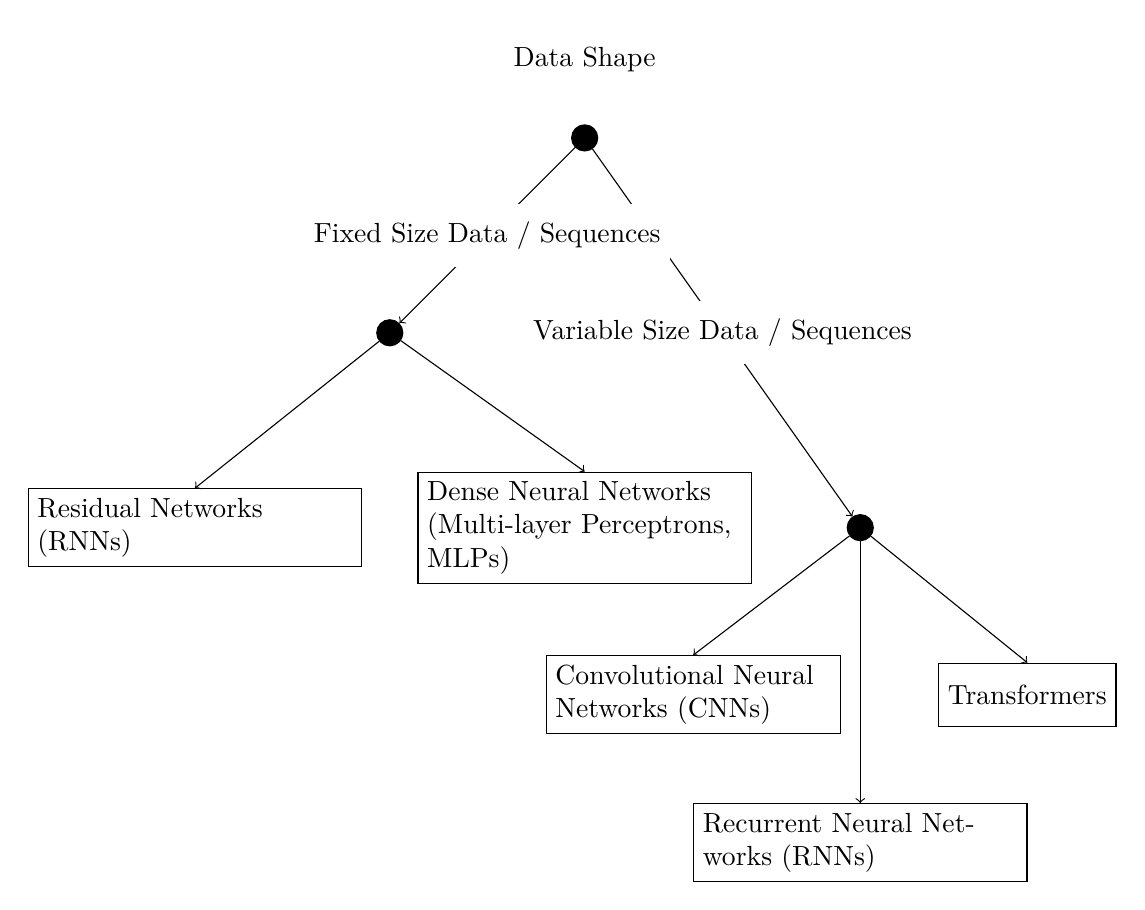
\begin{tikzpicture}
        \tikzstyle{every node}=[node distance=3.5cm,minimum height=0.8cm]
        % data shape
        \node[draw,fill=black,minimum height=0.2cm,circle] (taskroot) at (0,0) {};
        \node[above of=taskroot, node distance=1cm] {Data Shape};

        % fixed input shape
        \node[draw,fill=black,minimum height=0.2cm,circle, below left of=taskroot] (fixed)  {};

        % ResNet
        \node[draw, below left of=fixed,text width=4cm] (resnet)  {Residual Networks (RNNs)};
        \draw[->] (fixed) -- (resnet.north);

        % MLP
        \node[draw, below right of=fixed,text width=4cm] (mlp) {Dense Neural Networks (Multi-layer Perceptrons, MLPs)};
        \draw[->] (fixed) -- (mlp.north);

        % sequence
        \node[draw,fill=black,minimum height=0.2cm,circle,right of=mlp] (sequence) {};
        \draw[->] (taskroot) -- node[fill=white] {Variable Size Data / Sequences} (sequence);

        % this here to draw over above line
        \draw[->] (taskroot) -- node[fill=white] {Fixed Size Data / Sequences} (fixed);

        % CNN
        \node[draw, below left of=sequence,text width=3.5cm, node distance=3cm] (cnn) {Convolutional Neural Networks (CNNs)};
        \draw[->] (sequence) -- (cnn.north);

        % RNN
        \node[draw,below of=sequence,text width=4cm, node distance=4cm] (rnn) {Recurrent Neural Networks (RNNs)};
        \draw[->] (sequence) -- (rnn.north);

        % Transformer
        \node[draw,below right of=sequence, node distance=3cm] (transformer) {Transformers};
        \draw[->] (sequence) -- (transformer.north);

    \end{tikzpicture}
    \vspace{1cm}
    \captionsetup{parskip=7pt}
    \caption[Fixed vs variable input shape]{Neural network variants which support variable input shape.

    Due to their construction, MLPs and ResNets are restricted to a fixed input shape, and so can only be trained and used on data that is of a fixed size, such as tabular data, or data that has been processed into a fixed size by re-sampling, chunking etc.

    RNNs, CNNs and Transformers can accept variable length data, each with their own tradeoffs. They are typically more suitable for data that is naturally of variable size/length, such as text, audio or images.}
    \label{fig:ontology-input-shape}
\end{figure}

\begin{figure}
    \centering
    \begin{tikzpicture}
        \tikzstyle{every node}=[node distance=3.5cm,minimum height=0.8cm]

        % dataset type
        \node (datasettype) {Dataset Type};
        \node[draw, below of=datasettype] (seq) {Sequence Prediction};
        \draw (datasettype) -- node[fill=white] {Un-labeled} (seq);

        % input shape
        \node[right of=datasettype] (inputshape) {Data Shape};

        % loss
        \node[right of=inputshape] (loss) {Loss Functions};

        % angles
        \node[draw,fill=black,minimum height=0.2cm,circle,below of=loss,xshift=1.5cm] (angles) {};
        \draw (loss) -- node[fill=white] {Angles} (angles);

        \node[draw,fill=white,below of=angles,node distance=2.5cm, xshift=-2cm] (amse) {Squared Angular Error};
        \draw (angles) -- (amse.north);

        \node[draw,fill=white,below of=angles,node distance=2.5cm, xshift=2cm] (vonmises) {Von-Mises NLL};
        \draw (angles) -- (vonmises.north);

        \node[draw,fill=white,below of=loss,node distance=4.5cm,xshift=-1.5cm] (cat)  {Categorical};
        \draw (loss) -- node[fill=white] {Discrete} (cat.north);

        % transformer (here because needs to draw above a line)
        \node[draw, below of=inputshape] (transformer) {Transformer};
        \draw (inputshape) -- node[fill=white] {Sequences} (transformer);


        % chapter 4: arbitrary order sampling
        \node[draw,fill=white,text width=5cm] (chapter4) at (0,-8cm) {\textbf{\Cref{C:a-o-sampling}}: Arbitrary order sampling on MNIST};

        % chapter 6.2: transformer for hand pose prediction
        \node[draw,fill=white,text width=5cm] (chapter62) at (2.5cm,-10.5cm) {\textbf{\Cref{C:hand-model}, \Cref{S:mean-model}}: Predicting the next frame in a hand animation};

        % chapter 6.3: probabilistic model for hand pose prediction
        \node[draw,fill=white,text width=5cm] (chapter63) at (8cm,-10.5cm) {\textbf{\Cref{C:hand-model}, \Cref{S:prob-model}}: A flexible probabilistic model for hand motion prediction};

        \begin{pgfonlayer}{bg}
            \draw ([xshift=-4pt]seq.south) -- ([xshift=-4pt]chapter4.north);
            \draw ([xshift=-4pt]transformer.south) -- (chapter4.north);
            \draw (cat.south) -- ([xshift=4pt]chapter4.north);

            \draw (seq.south) -- ([xshift=-4pt]chapter62.north);
            \draw (transformer.south) -- (chapter62.north);
            \draw (amse.south) -- ([xshift=4pt]chapter62.north);

            \draw ([xshift=4pt]seq.south) -- ([xshift=-4pt]chapter63.north);
            \draw ([xshift=4pt]transformer.south) -- (chapter63.north);
            \draw (vonmises.south) -- ([xshift=4pt]chapter63.north);
        \end{pgfonlayer}

    \end{tikzpicture}
    \vspace{1cm}
    \captionsetup{parskip=7pt}
    \caption[Where my work sits.]{The later work in this thesis sits focuses on learning un-labeled sequence data with transformers, in two different domains.

    In \Cref{C:a-o-sampling}, I train a transformer-based probabilistic model which can be used as a gaussian process for predicting pixels on the MNIST dataset.

    In \Cref{C:hand-model}, I train a transformer-based model on the ManipNet hand motion dataset. \Cref{S:mean-model} focuses on a deterministic model, while \Cref{S:prob-model} focuses on a probabilistic model.}
    \label{fig:ontology-context}
\end{figure}

\TODO{ Use the correct terminology for " Regression (\textit{implicit} MLE)" and "Parameter regression (\textit{explicit} MLE)"}

The choice of training objective affects the settings in which a model can be used, which theoretical properties we get from it, and more.

The simplest kind of training objective is regression. When we train a model with a regression objective it learns to predict the expected value of the output. Regression is characterized by using an error function as the loss, for example \textit{mean-squared-error}:
\newcommand{\mse}{L_{\text{MSE}}}
\begin{align}
\label{notation:mse}
\begin{split}
    \fdef{\mse}{\R^{N×D}×\R^{N×D}}{\R} \\
    \mse&(y, \hat{y})_{ni} ≝ \frac{1}{N} \sum_n\left[ \sum_i (y_{ni} - \hat{y}_{ni})^2 \right]
\end{split}
\end{align}
This function sums the error over the \textit{feature} dimension $D$ and averages the error over the \textit{batch} dimension $N$ \footnote{Averaging has no effect on the optimization, it is simply that dividing by the batch and/or sequence length means that the loss value remains in the same range independent of the batch size or sequence length.}. Training a model by minimising this loss function, is equivalent to maximising the likelihood of a Gaussian distribution. Given input $x$, the model output $y = f(x)$ can be interpreted as $\E[p(y|x)]$.


\section{Auto-regressive models}

\TODO{ Formulation of auto-regressive models and sampling }

\TODO{ Things we can do with an auto-regressive model }

\section{Animation}


\section{Angle representations}

\TODO{ Quaternions and unitary / complex matrices }

\chapter{Understanding Transformers}
\label{C:transformers}

Many of the recent amazing results in deep learning have been achieved with a class of neural networks called \textit{transformers}, which were introduced and named in "Attention Is All You Need", Vaswani et al. 2017 \cite{attention-is-all-you-need}. The distinguishing feature of these models is using one or more \textit{attention} layers to enable information propagation between elements in sequence data. Since 2017, a large number of transformer variants have been developed, and in this chapter I seek to understand this class of models at a broader level. I will discuss:

\begin{itemize}
    \item The unique properties of the attention operation, which include working with sequences of any length without changing the weights, being able to be computed in parallel across the sequence during training, and being invariant to the order of the inputs.
    \item The different variants of transformers, namely encoder-only, decoder-only, and encoder-decoder models.
    \item The variety of different tasks that these model are trained on and used for, building up to the next chapter where I introduce an extremely generic gaussian-process-like task.
\end{itemize}

Firstly, I will discuss the operation that under-pins transformers -- attention.

\section{The Attention Operation}

Attention is a biologically-inspired mechanism that allows a model to receive inputs from distant parts of the input data, weighted by the \textit{attention weight} given to those inputs, which is typically computed from the data itself. This has proven extremely useful for diverse tasks including machine translation, image generation, and more. In this section I will describe the attention operator.

Attention has a number of useful properties which come from its mathematical construction, such as permutation-invariance in the inputs.

\subsection{Mathematical Definition}

An attention operation is of the following form, using short summation notation, where $\sigma$ is the \textit{softmax} operator (see \ref{eqn:softmax})
\begin{gather*}
    \nfdef{f_{\text{attn}}}{\R^{M×D}×\R^{N×D}×\R^{N×V}}{\R^{M×V}}
\end{gather*}
\vspace{-10pt}
\begin{equation}
\label{eqn:attn}
\begin{split}
    f_{\text{attn}}(Q, K, V)_{mv} ≝ \sum_n \left[\sigma\Big(\sum_d Q_{md} K_{nd}\Big) _{mn} V_{nv} \right]
\end{split}
\end{equation}%
\begin{gather*}
    Q ∈ \R^{M×D}, K ∈ \R^{N×D}, V ∈ \R^{N×V} \\
    M, N, D, V ∈ \N
\end{gather*}\vspace{-10pt}\\
The innermost multiplication of $Q$ and $K$ in the above equation is simply the expanded form of inner product (dot product) between vectors $Q_m$ and $K_n$. This operation however is not inherent. Instead of the inner product, we can substitute any kernel function $k(q, k)$
\begin{equation}
\label{eqn:attn}
\begin{split}
    f_{\text{attn}}(Q, K, V)_{mv} ≝ \sum_n \left[\sigma(k(Q_m, K_n)) _{mn} V_{nv} \right]
\end{split}
\end{equation}%
However, substituting a different kernel function is not usually done because the inner product is the most natural choice, and is efficient to compute.

For clarity, the expanded form of the attention computation, resulting in the unnormalized attention weights $A$, for an arbitrary kernel function $k$, is as follows:
\begin{align*}
A_{mn} = k(Q_m, K_n)
&= \begin{bmatrix}
    k(Q_{1}, K_{1}) & k(Q_{1}, K_{2}) & \cdots & k(Q_{1}, K_{N}) \\
    k(Q_{2}, K_{1}) & k(Q_{2}, K_{2}) & \cdots & k(Q_{2}, K_{N}) \\
    \vdots & \vdots & \ddots & \vdots \\
    k(Q_{M}, K_{1}) & k(Q_{M}, K_{2}) & \cdots & k(Q_{M}, K_{N})
\end{bmatrix} \\
\text{or when\ } k(a, b) = a \cdot b &\text{, then} \\
&= \begin{bmatrix}
    Q_{1,1} & Q_{1,2} & \cdots & Q_D \\
    Q_{2,1} & Q_{2,2} & \cdots & Q_D \\
    \vdots & \vdots & \ddots & \vdots \\
    Q_{M,1} & Q_{M,2} & \cdots & Q_D
\end{bmatrix} \begin{bmatrix}
    K_{1,1} & K_{1,2} & \cdots & K_D \\
    K_{2,1} & K_{2,2} & \cdots & K_D \\
    \vdots & \vdots & \ddots & \vdots \\
    K_{N,1} & K_{N,2} & \cdots & K_D
\end{bmatrix}^T \\
&= Q K^T .
\end{align*}

We can see that the attention weights $A$ have shape $M×N$. This is the primary drawback of the attention operation. $M$ and $N$ are typically both large, and the attention weights take $O(MND)$ time to compute (assuming dot product attention), and $O(MN)$ space to store. Despite this drawback, the attention operation has proven extremely useful in a variety of tasks. There are many different ways to address this but I will not discuss them.

\subsection{Permutation-invariance with respect to $K$ and $V$}

The first interesting property of attention is that it is permutation-invariant with respect to the key and value inputs. This property is more or less useful depending on the task. For example, in the case of graphs, or sets of heterogeneous values, there may not be a natural ordering in which to process the inputs. In this case, we do not have to introduce any artificial ordering. (However, when \textit{sampling} outputs, we typically still need to decide on some order. I will discuss this in more detail in \Cref{C:a-o-sampling}).

This property is due to the construction of the attention operator. We can see that the output $O_m$ corresponding to a query vector $Q_m$ is independent of the order of the key and value vectors $K_n$ and $V_n$, because the summation across $n$ is commutative:
\begin{align}
\label{eqn:attn-perm-invariance}
\begin{aligned}
    O_m &= \sum_n V_n \sigma(A_{m})_n
\end{aligned}
\end{align}

\subsection{Permutation-equivariance with respect to $Q$}

Relatedly, attention is also permutation-\textit{equivariant} with respect to the query inputs. Equivariance means that the value of the output $O_m$ is dependent on the value of the query vector $Q_m$, but independent of the order of all \textit{other} query vectors $Q_{m'}$, $m' ≠ m$.

For example, let us imagine we have a sequence of four key \& value inputs $[K_1, K_2, K_3, K_4]$, and $[V_1, V_2, V_3, V_4]$, and a sequence of three query inputs $[Q_A, Q_B, Q_C]$ which when passed into an attention operation, produce three outputs $[O_A, O_B, O_C]$. First, due to the first property (invariance in $K$ and $V$), if we swap for example the inputs $K_1$ \& $V_1$ with $K_3$ and $V_3$, the output sequence will remain $[O_A, O_B, O_C]$. Second, if we swap the inputs $Q_A$ and $Q_C$, the second property (equivariance in $Q$) means that the output sequence is correspondingly transformed to $[O_C, O_B, O_A]$.

This property is due to the fact that softmax operation is equivariant to the order of its inputs, which we can see from the construction in \Cref{eqn:softmax}.

This property of attention stands in contrast to the two main other methods used to process sequence data, convolution (CNNs) and recurrence (RNNs). Neither of these operations are permutation invariant or equivariant with respect to their inputs.

\subsection{Dynamic length inputs}

The second (and most useful) property of attention is that it can be used to process inputs of dynamic length. We can again see why this is the case from \Cref{eqn:attn-perm-invariance}. The softmax operation normalizes the attention weights, which causes the resulting summation of vectors $V_n$ to be a convex combination. The resulting output $O_m$ will therefore sit within the convex hull of the vectors $V_n$. This means that the output $O_m$ will be a ``valid'' output regardless of the length of the input sequence $K_v$.

\subsection{Parallel computation}

The third property of attention is that it can be computed in parallel across the inputs sequence during training. At all steps of the attention computation except the softmax operation, there are no dependencies between neighbouring elements of the tensors. This stands in contrast to RNNs, where the outputs for one position in the sequence depend on the previous outputs.

The fact that attention can be computed in parallel is a very useful property, since while the operation requires $O(MN)$ in time and space, if we can utilize bigger GPU hardware the real-time cost reduces to $O(1)$ (assuming sufficient memory capacity, compute capability, and also GPU memory bandwidth, which is often the limiting factor \cite{multi-query-attn}.) The attention logits $A_{mn}$ can be computed entirely in parallel. The softmax operation depends on all previous attention logits across the key-value dimension $N$, which requires cross-talk between GPU units but does not prevent parallel computation. The final computation for the outputs $O_m$ can also be computed in parallel.

So attention is a operation with a number of useful properties. Now we will see how it is used to build a variety of models capable of solving a variety of tasks with sequence data.

\section{Basic components of transformers.}

An attention operation model does not itself make a neural network. It is simply a building block that can be used to construct a neural network.

A transformer model puts attention operations together with MLP blocks similarly to in residual networks (ResNets). Without MLP blocks as non-linearities, the outputs of an attention operation are linear functions of the inputs, since the softmax is only used to compute coefficients when summing the values. Because the weights are convex (sum to 1), the output vectors of an attention operation are convex combinations of the value vectors, and will always sit within the convex hull of the value vectors. (However, note that the outputs are non-linear functions of the inputs, due to the fact that the weights are also computed from the inputs). Attention-only we would like to be able to apply non-linear transformations to the value vectors. MLP blocks are used to introduce additional non-linearities into the model.

In \Cref{fig:residual-block} we can see a diagram of a typical residual block in a transformer, combining an attention operation, a feed-forward layer, and a residual connection as in a ResNet.

\begin{figure}
    \centering
    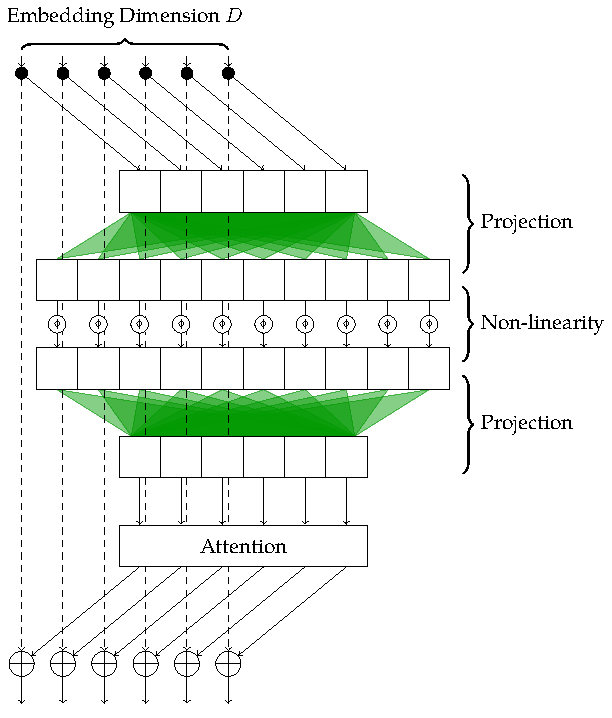
\includegraphics[]{figures/residual-block.pdf}
    \captionsetup{parskip=7pt}
    \caption[Typical residual block in transformer]{Typical residual block in transformer (with the $D$ dimension expanded, rather than the $N$ or $M$ dimension as usual.).

    In the MLP block, the sequence of residual latents are independently projected into a higher-dimensional space, where a non-linearity is applied, and then projected back down to the original dimensionality. The output of the MLP block is then projected into $Q$, $K$, and $V$ spaces, and the attention operation is applied. Finally, the results are added to the residual stream.}
    \label{fig:residual-block}
\end{figure}

Attention is computed from the three matrices (or sequences of vectors) $Q$, $K$ and $V$. In a neural network, these are each typically derived in some fashion from the inputs to the network. The most common way to do this is to use a learned linear transformation, which is simply a matrix multiplication followed by a bias term, for example
\begin{align}
\begin{aligned}
\label{eqn:attn-linear}
Q &= W_{Q} \X + \vb_{Q} \\
K &= W_{K} \X + \vb_{K} \\
V &= W_{V} \X + \vb_{V}
\end{aligned}
\end{align}


If we derive all three matrices from the same input $\X$, then $M = N$ and the attention operation is called a \textit{self-attention} operation. A diagram of this is shown in \Cref{fig:self-attn}. The blue shaded areas show the receptive field used when computing each output vector $x'_i$.

When Q and K are derived from separate sequences of feature/embedding vectors, then in general $M ≠ N$ and this is called \textit{cross-attention}. A diagram of this is shown in \Cref{fig:cross-attn}.

\begin{figure}
    \centering
    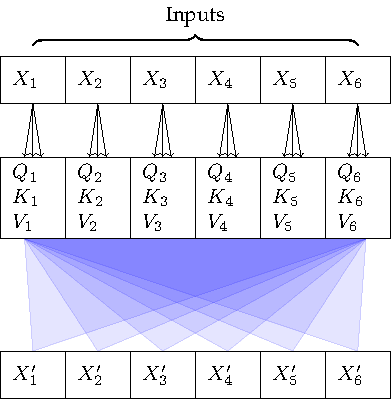
\includegraphics[]{figures/attn-1-self.pdf}
    \caption[Self-attention]{Full self-attention (bi-directional attention), as used in transformer encoders. The blue shaded regions show which inputs are used to compute each output. In full self-attention, all inputs are used to compute all outputs.}
    \label{fig:self-attn}
\end{figure}


\begin{figure}
    \centering
    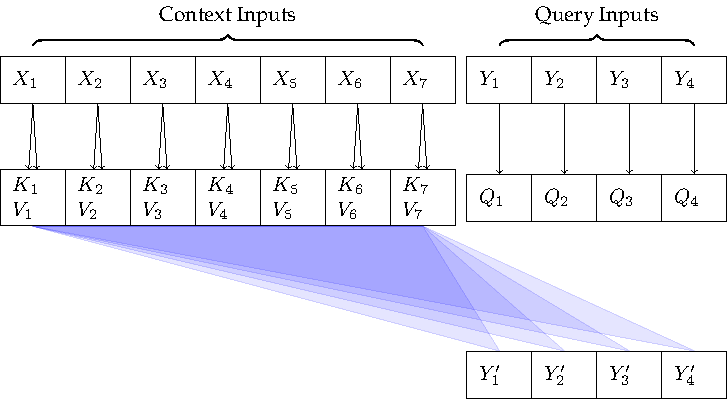
\includegraphics[]{figures/attn-2-cross.pdf}
    \caption[Cross-attention]{Cross-attention, as used in encoder-decoder models.}
    \label{fig:cross-attn}
\end{figure}

Since the introduction of transformers it is common to use \textit{multi-head} attention, which allows for multiple \textit{heads} which each perform an attention operation in parallel with smaller key dimensionality $D_{\text{head}} = \frac{D}{ n_{\text{heads}}}$.

The defining feature of a transformer model is that it has ``attention'' layers. However, there is not just one way to assemble these layers, and there is not just one way to train these models.

We can broadly split the transformer architecture variants into four categories: \textit{encoder-only} models, \textit{decoder-only} models, unified attention models, and \textit{encoder-decoder} models.

\subsection{Masked Sequence Modeling: Encoder-only models}
\label{ss:msm}

Arguably the simplest attention-based model architecture is encoder-only transformers. When used in natural-language-processing (NLP) they are known as bi-directional language models, because they allow information to flow in both directions. Examples are the BERT \cite{bert} language model family, Wav2Vec \cite{wav2vec} for speech, and SimMIM \cite{sim-mim} image model.

These models are trained on a sequence reconstruction task, called Masked Language Modeling (MLM), Masked Image Modeling (MIM), or more generally Masked Sequence Modeling, which I will discuss more in \Cref{ss:pretraining}.

These models are typically used for sequence understanding tasks and classification tasks, however they can also be used for generating sequences. The limitation of these kinds of models is that their pretraining task is not efficient for training these models to generate sequences. For generating sequences, an encoder model in conjunction with a \textit{decoder} model (see \Cref{ss:encoder-decoder}), or simply a decoder-only model.

\subsection{Sequence Prediction: Decoder-only models}
\label{ss:decoder-only}

A diagram of the decoder-only architecture, is shown below in \Cref{fig:decoder-only}. The distinguishing feature of a \textit{decoder} as opposed to an encoder is that its attention layers are all causally-masked self-attention layers as in \Cref{fig:self-attn-causal}. These models are used for sequence prediction/generation, and trained via self-supervised learning.

Some examples of where we see this architecture in use are:
\begin{itemize}
    \item OpenAI's GPT-series \cite{gpt2, gpt3} language models.
    \item Latent code prediction (the ``prior'') in VQ-GAN \cite{vqgan}
\end{itemize}


\begin{figure}
    \centering
    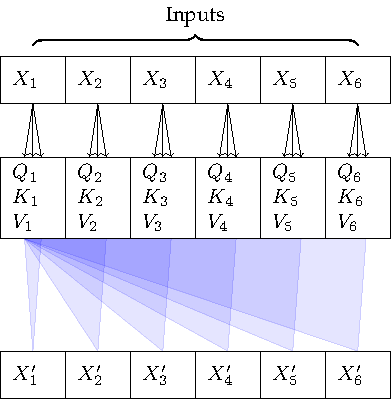
\includegraphics[]{figures/attn-3-causal.pdf}
    \caption[Self-attention with causal masking]{Self-attention with causal masking, (uni-directional attention) as used in transformer decoders during training. The blue shaded regions show which inputs are used to compute each output. In causal masking, only inputs to the left of the current output are used to compute the current output.}
    \label{fig:self-attn-causal}
\end{figure}

\begin{figure}
    \centering
    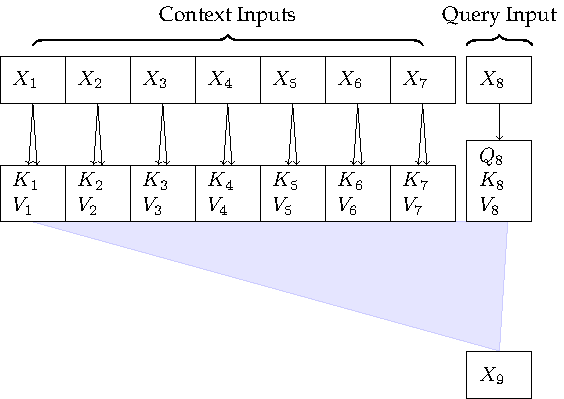
\includegraphics[]{figures/attn-4-partial.pdf}
    \caption[Partial self-attention]{Partial self-attention, as used during incremental autoregressive inference (in models with a decoder).}
    \label{fig:partial-self-attn}
\end{figure}


\begin{figure}
    \centering
    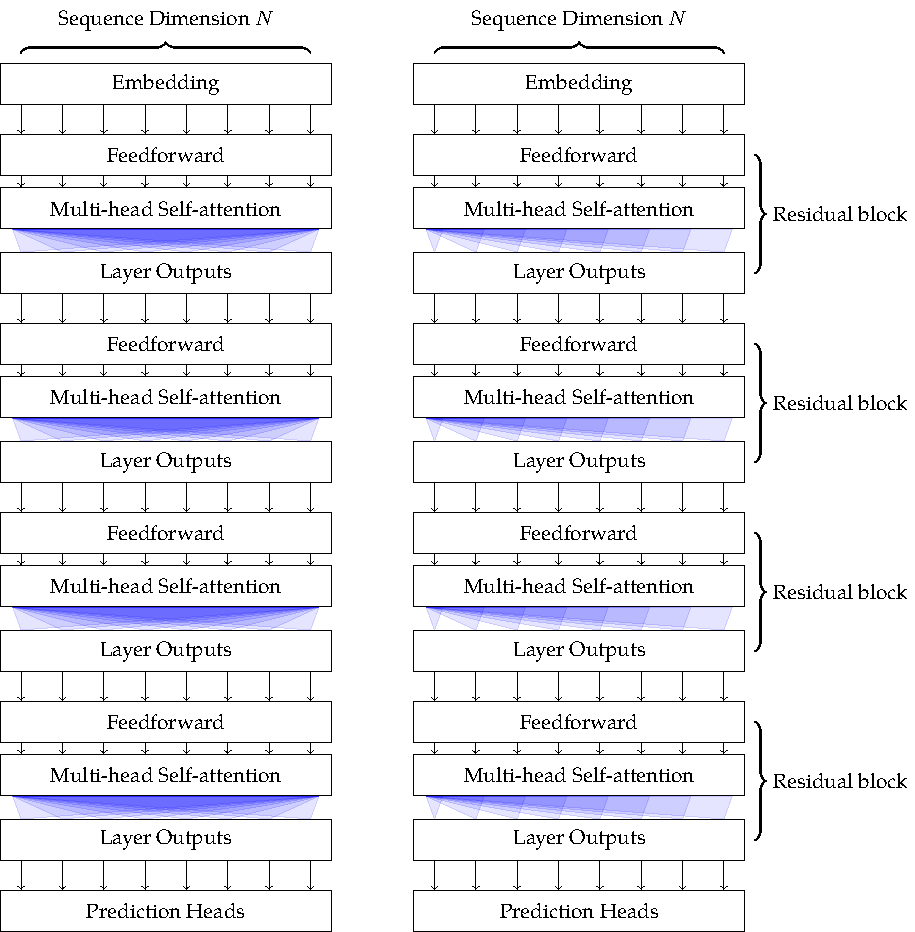
\includegraphics[width=1.2\linewidth]{figures/transformers.pdf}
    \caption[Transformer model]{Left: Encoder-only model. Right: Decoder-only model. Residual connections have been ommitted for brevity.}
    \label{fig:transformers}
\end{figure}


\subsection{Encoder-decoder models}
\label[]{ss:encoder-decoder}

When the transformer was introduced in \cite{attention-is-all-you-need}, the first architecture proposed was an encoder-decoder architecture. This is a model which has both an encoder and a decoder. The encoder is used to encode a sequence of \textit{conditioning} or \textit{context} inputs, and the decoder is used to generate the output sequence. The encoder and decoder are connected by cross-attention layers (see \Cref{fig:cross-attn}), which allow the decoder to attend to the encoded context sequence.

These are the most flexible class of model, because they allow predicting some outputs, or sequences of outputs, \textit{given} some inputs.

Examples of this are the original transformer architecture \cite{attention-is-all-you-need}, the BART \cite{bart} model, and more recently Google's Parti multi-modal text-to-image model \cite{parti}.

In \cite{attention-is-all-you-need}, they train an encoder-decoder architecture for text translation. Their architecture takes one sequence of text tokens (if you are wondering what text tokens are, I will discuss input formats in the next section) in language A as conditioning input, then auto-regressively samples a target sequence in a second language B. The two languages may have very different word orderings or numbers of words to each other, but the cross-attention operation introduces no bias towards aligned word orderings or even word counts.

\subsection{Unified attention models}

\begin{figure}
    \centering
    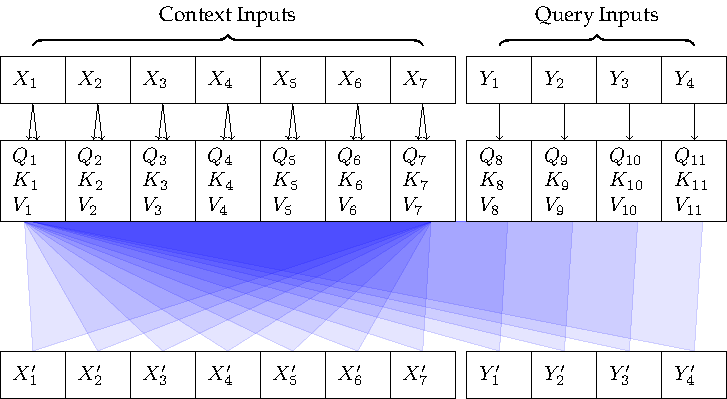
\includegraphics[]{figures/attn-5-unified.pdf}
    \captionsetup{parskip=7pt}
    \caption[Unified attention]{Unified self- and cross-attention, from \cite{unilm}.

    Bi- and uni-directional attention can be performed with the same attention layers with careful masking, allowing the same model to be trained on any mixture of pre-training tasks.

    The ``encoder'' outputs $X'$ are computed with full self-attention, and the ``decoder'' outputs $Y'$ are computed with full attention with respect to $X$ and causal attention with respect to $Y$.}
    \label{fig:unified-attn}
\end{figure}

As we see in \ref{fig:unified-attn}, there are actually two ways we might include information from the encoded sequence into the decoded sequence. In the first, which is used in most encoder/decoder models including the original, all the layers of the encoder are computed fully, and the final encoded sequence is provided to the decoder at all layers via cross-attention. In the second, the encoder is separated from the decoder only by correct application of masking in the attention layers, and is only computed up to the layer which is being decoded at.

This second scheme is called ``unified'' attention, eg. \cite{unilm,t5}.

\begin{figure}
    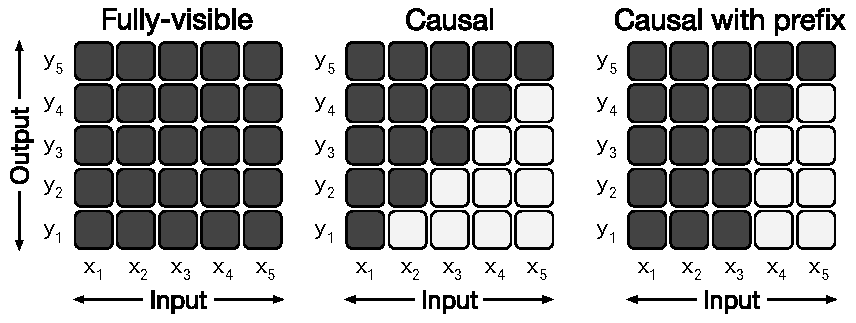
\includegraphics[width=\linewidth]{figures/attention_masks.pdf}
    \caption[Attention Masks]{Masking in unified attention layers \cite{unilm,t5}. The bi- and uni-directional attention can be performed within a single attention layer.}
    \label{fig:unified-masking}
\end{figure}

The different layouts that can be used are shown in \Cref{fig:unified-masking}.

The first method is more efficient because the attention matrices of the encoder and the decoder are split, using $O(N^2 +M^2)$ memory rather than $O(N^2M^2)$. However, the second method is conceptually simpler and is better when the trained model will be used for fine-tuning/transfer learning \cite{t5}., because it uses the decoder to attend to the encoded sequence at any layer, and not just the final layer. This is useful for tasks such as image captioning, where the decoder may want to attend to the encoded image at multiple layers, and not just the final layer.

Transformer models trained on a mix of pre-training tasks using unified attention architecture are known as T5 models (\textbf{T}ext-\textbf{T}o-\textbf{T}ext \textbf{T}ransfer \textbf{T}ransformers) \cite{t5}.



% attention
% transformer architectures
% pre-training types

In the next chapter (\Cref{C:a-o-sampling}) I experiment with a new pre-training task, which is a variation on auto-regressive sequence modeling, which I call \textit{arbitrary-order autoregressive pretraining}, which I will later apply to hand motion prediction.

\chapter{Sampling Sequences In Any Order}
\label{C:a-o-sampling}

In this chapter I investigate learning auto-regressive transformers to generate pixels of the MNIST dataset. By changing the model architecture and training procedure, I show that we can learn to generate pixels in any order, including dynamically choosing the order of the pixels while sampling. In effect, we learn a model that can be used as a Gaussian process on this dataset.

In particular, I compare the following sampling orders with my model:
\begin{itemize}
    \item Left-to-right, top-to-bottom
    \item Random
    \item Highest-entropy-first
    \item Lowest-entropy-first
\end{itemize}

Contrary to my hypothesis that a lowest-entropy-first sampling order would result in the best samples, I find that this biases the samples towards images with large amounts of empty background, such as images of 1s. Correspondingly, a highest-entropy-first sampling order biases the samples towards images of 8s and 9s. In the discussion, I argue this occurs because the criterion we are selecting for introduces a bias, and I characterise this bias.

\section{Introduction}

% sampling high-dimensional data
% choosing the order to sample in for higher-quality samples

\section{Background}

When modeling data, it is often useful to have a \textit{probabilitic} model of the data, rather than a deterministic model. This allows us to quantify uncertainty about the model outputs, sample from the model, and avoid problems with multi-modal distributions. However, when the data we are modeling is high-dimensional, probabilistic models often become computationally expensive or intractable.

\subsection{Autoregressive models}

For example, let us imagine we are modeling a sequence of $N$ observations $\x_i \in \R^D$, $1 ≤ i ≤ N$ (each observation is a $D$-dimensional vector). To represent the joint distribution over this data, even with a simple gaussian distribution requires $DN + (DN)^2$ parameters ($DN$ means, plus a $DN \times DN$ covariance matrix). If $N$ is large, this is a very large number of parameters, but still manageable.

A gaussian however is limited in its ability to model the data. For example, it cannot model multi-modal distributions. To model multi-modal distributions, we could use a mixture of gaussians, but this increases the number of parameters even further, to $(DN + (DN)^2)K + K$, where $K$ is the number of mixture components, making sampling and inference much more expensive.

In general, the more expressive the family of distributions we use to model the data, the more parameters we need to represent the distribution and the more expensive it is to sample from the distribution.

There are a few main approaches to address this problem, which I show below:

\begin{itemize}
    \item Discretization
    \item Independence assumptions
    \item Auto-regressive factorization
\end{itemize}

One approach to managing the intractibility of high-dimensional data is to discretize the data, and then model it with a categorical distribution. For example, we can use a clustering algorithm to learn a series of $K$ points within our $DN$-dimensional space, and then form a discrete distribution over these points. A discrete distribution over $K$ points has $K-1$ free parameters, so this approach reduces the number of parameters from $(DN)^2$ to $K-1$, and makes sampling and inference more efficient. However the discretization changes the domain of the data, which may not always be useful. Additionally, the larger the domain, the more cluster points we need to use, and we might not be able to find a good clustering of the data.

Independence assumptions are another way to reduce the number of parameters. For example, we could assume that the observations $\x_i$ are independent, and then model the sequence as a product of $N$ independent $D$-dimensional distributions. For a Gaussian, this means fixing parts of the co-variance matrix, and we often reduce to having a single variance parameter. A single variance parameter reduces the number of parameters from $(DN)^2$ to $DN$, but it also makes the model less expressive. For sequence data, this assumption is almost never valid along the sequence dimension, so this approach is not very useful.

Auto-regressive factorization is a third approach to reducing the number of parameters. In this approach, we break down the joint distribution over the sequence into a product of conditional distributions, where each conditional distribution depends only on the previous observations. We then typically model all of these conditional distributions with the same model.

\begin{align}
    \label{eqn:ar-factorization}
    \begin{aligned}
        p(\x_1, \x_2, \ldots, \x_N) &= \prod_i^N p(\x_i | \x_1, \ldots, \x_{i-1})
             &= p(\x_1) p(\x_2 | \x_1) p(\x_3 | \x_1, \x_2) \ldots p(\x_N | \x_1, \ldots, \x_{N-1})
    \end{aligned}
\end{align}

When we use an auto-regressive model to predict sequences, we usually choose some fixed order for this decomposition. For data with a temporal dimension, this is usually first-to-last, which is usually natural because the real process that generated the data had a causal structure in the temporal dimension.

However, it is valid to perform the decomposition in any order, for example choosing a random permutation of the sequence(s):

\begin{align}
    \label{eqn:ar-factorization-random}
    \begin{aligned}
        J = {5, 3, 9, 1, ..., N }
        p(\x_1, \x_2, \ldots, \x_N) &= \prod_{i \in J}
    \end{aligned}
\end{align}

In the case of data that does not have a temporal dimension, such as pixels in an image, or joint angles of a hand (within one frame), simple ordering may not always be the best. Also, some data may have very long sequences and latency requirements (such as character animation data), where it is expensive to generate the data in order, and we would instead like to generate only particular parts of the sequence.

\subsection{Dynamically-ordered auto-regressive sampling}

If we have an auto-regressive model of the appropriate form that has been appropriately trained, we can dynamically choose the order that we sample a sequence. The form of the model must be such the the data $\x_i$ can be split into two components `position' and `content' which we will represent with $x_i$ and $y_i$ respectively.

Given some seed sequence length $i$ we have input data $\x_{<i} = \{ (x_n, y_n) \mid n < i \}$. For each remaining position $x_n$, $n ≥ i$, we can compute the conditional distribution $p(y_n | x_n,  \x_{<i})$. This gives us $N$ conditionally-independent distributions each for a different $x_n$. We can choose any statistic of these distributions to select which one to sample from. For example, we could choose the distribution with the highest entropy, or the distribution with the lowest entropy, or the distribution with the highest mean, or the distribution with the lowest mean, etc. We can then sample from the chosen distribution to get the next $y_n$. Because we sample, we in principle do not change the distribution of results -- however in practice, we may change the distribution of results because of the way we choose the statistic. I will discuss this in \Cref{S:a-o-discussion}.


\subsection{Training task and input formats}
\label{ss:transformer-inputs}

As we saw before in \Cref{s:pretraining} we have two main tasks for training a transformer model:

\begin{itemize}
    \item \textbf{Masked Sequence Modeling}, which we use to train models with bi-directional attention - predict the masked out tokens.
    \item \textbf{Autoregressive Sequence Prediction}, which we use to train a model that uses causal attention - predict the next token in sequence.
\end{itemize}

As we saw in the above section, transformers can have their input provided as (position, content) pairs, which naturally maps onto the above auto-regressive factorization. However, not all training tasks will result in a model that learns to use the position information in this way.

More generally, the input to a transformer is some kind of $D$-dimensional embedding. When specifiying both the input and content , we first project the which is unique among the input set, such as special ``BEGIN'' or ``CLASS`` tokens.

Both the attention layers and feed-forward layers are invariant to permutations of the input sequence. Additionally, there is no requirement that the input set be contiguous in the sequence dimension - there can be (potentially large) gaps, with no change to to the structure of the model (however, the model must be trained for the particular problem still).

As a result of being invariant to permutations, and working with non-contiguous sequences, we can present many different kinds of sequence prediction tasks to a transformer that we could not easily present to other models.

\begin{itemize}
    \item A Recurrent Neural Network (RNN) can be given sequences with gaps (using the same position/content encoding), but is not invariant to the order of the "previous token" conditioning data, which must be incorporated first in some particular order.
    \item A convolutional or dense neural network applied to the input including the sequence dims (ie. not ``pointwise'') is neither invariant to the order, nor can be applied to sequences with gaps.
\end{itemize}

In the next section I describe some tasks we might want to perform with these unique abilities of a transformer.


\section{Hypothesis}
\label{s:a-o-hypotheses}

Using the above two methods ``triples'' and ``pure-query-decoder'' models, I investigated a hypothesis about selecting a better sampling order on a toy dataset.

The hypothesis was as follows.

Assume that using the above methods, we can choose a dynamic ordering in which to sample a sequence at inference time. In particular, one of the ways we can do this is by evaluating the \textit{entropy} of all candidate positions, then sampling from the one with either the lowest or the highest entropy.

When auto-regressively sampling pixels to produce MNIST images, using a ``lowest-entropy-first'' ordering might produce visually better results than a ``highest-entropy-first'' ordering.

\section{Method: Details of experiments.}

To investigate this hypothesis, I developed and trained a transformer model on two separate tasks - one for predicting the next pixel in a sequence, and one for predicting a random. I compared a variety of architecture choices and training methods. I show the results of these experiments as figures for subjective evalutaion throughout this chapter.

\subsection{Data}

This series of experiments uses the MNIST dataset, which is a set of 28x28 grayscale images of handwritten digits. The dataset is split into a training set of 60,000 examples, and a test set of 10,000 examples. Each image is labeled with the digit it represents, from 0 to 9, but I did not use this information in my experiments. Each pixel is represented as a value between 0 and 255, where 0 is black and 255 is white.

Instead of representing full 256 colors, I used a 2-bit representation, where each pixel is represented as a value between 0 and 3. I discretized the 256 colors into 4 colors using a learned k-means clustering over the whole dataset. This was to simplify the form of the distribution that the model would output, and remove any complextity here as an additional variable to debug. I found that 4 colors was the smallest representation that gave good visual quality when the images were reconstructed.

To turn MNIST data into a sequence prediction task, I used the following procedure. For each image, I created a sequence of 28x28 pairs, where each pair is a pixel position and a pixel value. The pixel position is represented as a pair of integers, where the first integer is the row number, and the second integer is the column number. The pixel value is represented as a single integer, where 0 is black, 1 is dark gray, 2 is light gray, and 3 is white.


The tasks the model was trained on are then both as follows: ``Given a sequence of pairs, and a target position, predict the value of the pixel at that position.''

However, in the first task the pairs are presented in a contiguous forward-only order, and in the second task the pairs are presented in a non-contiguous, random order. In the random order task, many unique permutations of each training image are created using on-the-fly data augmentation. This is to ensure that the model is not overfitting to a specific ordering of the training data.

We can see examples of this in \cref{fig:mnist-task-examples}.

\begin{figure}
    \centering
    
\includegraphics[width=0.5\textwidth]{figures/examples-sequential.png}
    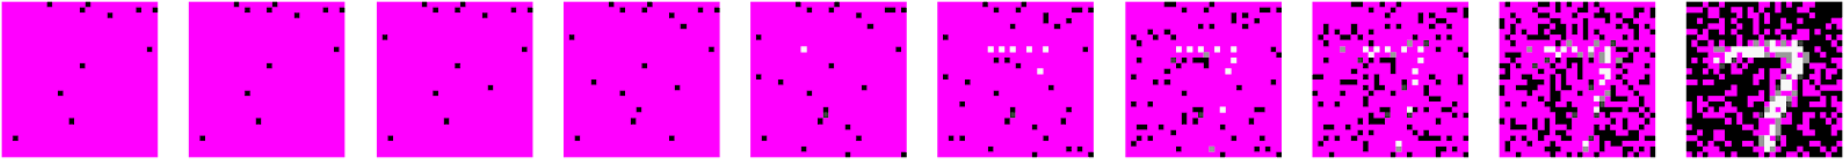
\includegraphics[width=0.5\textwidth]{figures/examples-random.png}
    \caption[Examples of the two MNIST training tasks]{Examples of the two tasks, showing input sequences with progressively more pixels filled in. (Pink means the pixel was not provided). Top: Pixels are presented in a contiguous forward-only order. Bottom: Pixels are presented in a non-contiguous, random order.}
    \label{fig:mnist-task-examples}
\end{figure}

In addition to the above encoding I experiment with two slightly different pre-training tasks for the ``random-order'' task. In the first, I use the ``Masked Sequence Modeling'' task, where I mask out a random subset of the pixels in the image, and the model is trained to predict the masked out pixels. In the second, I use a ``Autoregressive Sequence Prediction'' task, except with additional positional information, where the model is given both the positional information of the current pixel and the next pixel when predicting the value of the next pixel.

\subsubsection{Arbitrary order decoder-only transformer using input triples}
\label{sss:decoder-only-triples}

This is a variant on auto-regressive sequence modeling that I developed for this project. Let us recall causal/autoregressive pretraining from the previous chapter. (See \Cref{fig:pretraining-causal}) Recall that these predict the next input from the previous input, conditioned on the rest of the sequence via their attention layers.

We can represent the input as
$$
   \x = (y_{<i}, x_{<i}) = ( \{ y_i, y_{i-1}, ..., y_1 \}, \{ x_i, x_{i-1}, ..., x_1 \} )
$$
where $i$ represents the position of a token, and $x$ represents the value of a token. When predicting the next input from the previous input, the model typically infers the next position from the previous position during the process of predicting.

However, if we are to use random positions, the model is not able to infer the position to predict. We instead construct an input sequence in the following way
$$
   \x = (x_{<i+1}, y_{<i}, x_{<i}) = ( \{ x_{i+1}, x_{i}, ..., x_2 \}, \{ y_i, y_{i-1}, ..., y_1 \}, \{ x_i, x_{i-1}, ..., x_1 \} )
$$.

By providing the input as (target position, input position, input value] triples instead of [input position, input value] pairs (in which the target is implicit), we allow the model to predict the next input value without inferring the next position.

If our sequence is presented in contiguous-forward-only ordering, $i$ is always paired with $i+1$ and we do not introduce any new information. However, since we create a sequence with an arbitrary order during training, the model learns to utilize this information.

Then, at inference time we can choose $x_{i+1}$ to be any position that we want the model to predict next, by constructing the following triple $(x_{i+1}, y_i, x_i)$ and appending it to the rest of the previous tokens.


\subsection{Models}

\subsubsection{Architecture choices}

All model architectures shown here are transformer models, but they vary in the following ways:

\begin{enumerate}
    \item Absolute vs relative positional encodings
    \item Whether or not they include a ``query decoder''.
    \item If so, whether this decoder has a pooled input or not.
    \item Number of layers, embedding dimensionality etc.
\end{enumerate}



\section{Discussion}
\label{s:a-o-discussion}

As we can see in \Cref{fig:order-comparison}, the ``lowest-entropy-first'' ordering produces distinct images from the ``highest-entropy-first'' ordering. However, neither are as good as the ``random'' ordering.

Why do the ``lowest-entropy-first'' and ``highest-entropy-first'' orderings produce such different results? Why should they be different from the ``random'' ordering?

If the model has perfectly learned the true distribution of the data, then all orderings should produce the same results. However, the model is not perfect, and the ``random'' ordering is the only one that is not biased by the model's imperfections.

When we select a dynamic ordering based on the model's predictions, we are introducing a bias into the model's predictions. Let us examine this bias in more detail.

Let us imagine that the model outputs a gaussian =- more specifically it outputs estimates of the parameters $\mu$ and $\sigma$ of the true conditional distribution $p(y_i \mid x_i, y_{<i}, x_{<i})$. Then, also assume we can approximate the the fact that the model is imperfect by adding gaussian noise to the model's output, $\mu + \epsilon_\mu$ and $\sigma + \epsilon_\sigma$, where $\epsilon_\mu \sim \N(0, v_\mu)$ and $\epsilon_\sigma \sim \N(0, v_\sigma)$, for some small $v_\mu$ and $v_\sigma$. Let the model's output distribution be $q(i) = \N(y_i | x_i, y_{<i}, x_{<i}, \mu + \epsilon_\mu, \sigma + \epsilon_\sigma)$.

If we select the next position $i$ randomly, then when we sample $y_i \sim q(i)$, since the means of the error terms $\epsilon_\mu$ and $\epsilon_\sigma$ are both 0, the expected value of $y_i$ remains $\mu$.

However, when we select the next location $i$ to sample based on the entropy of $q(i)$, we select the location among many which has the highest (or lowest) variance $\sigma + \epsilon_\sigma$. On average, we will select a position with both high contribution from $\sigma$, \textbf{and} high contribution  from $\epsilon_\sigma$. Because of the high $\epsilon_\sigma$ term, this selection biases us towards sampling from distributions where the model is more uncertain than in the true distribution. We will therefore draw samples that are on average \textbf{less likely} in the true distribution. I.e. $\E[p(y_i \mid x_i, y_{<i}, x_{<i})] < \E[q(i)]$. To summarize, when we select an $i$ because the corresponding $q(i)$ has high entropy (variance), and then sample from this distribution, we will produce a pixel with a value that has $p(y) < q(y)$. The reverse is true for the ``lowest-entropy-first'' ordering. This is the bias that we are introducing into a \textit{single} prediction from the model.

I claim this same reasoning applies for the discrete case which I actually used in the experiment -- we can add an $\epsilon$ term to the logits, which when selecting for high entropy, pushes them towards the uniform distribution, and when selecting for low entropy, pushes them away. It so happens that on MNIST, this typically means the pixel will be brighter.

As we repeat this process, we will produce some pixels that are on average brighter than the true sequence. When the model is conditioned on these, it will generally infer that the remaining pixels should be brighter as well. This is why the ``highest-entropy-first'' ordering produces images that are as a whole brighter than the ``lowest-entropy-first'' ordering, and why both are shifted away from the ``random'' ordering.

\chapter{Angles, Joints and Hands}
\label{C:angles-joints-hands}

This next chapter discusses the development of a model to predict motion of a human hand. To understand the model and some of the implementation choices, it is necessary to understand the anatomy of the hand, and how the many degrees of freedom of the hand can be represented (paramaterized). This chapter discusses the different ways to parameterize angles, 3D rotations, and collections of many joints. It also introduces some loss functions for training neural networks where the input and output are angles.

\section{Representing Angles}

In toplogical terms, an angle is a point on the unit circle, aka the 1-sphere $S^1$. In the context of 3D rotations, an angle is a rotation around a single axis. We typically use either of two representations for angles: A single number or a 2D unit vector.

Representing an angle as a single number (in either radians or degrees) is the most common representation. It is simple and addition between angles represented in this way is well defined.

The other representation is the unit vector representation. In this representation, an angle $a$ is represented by a 2D unit vector $v$
\begin{equation}
    v = \begin{bmatrix}x \\ y\end{bmatrix} = \begin{bmatrix}\cos{a} \\ \sin{a}\end{bmatrix}
\end{equation}.
This representation is useful for neural network implementations for two reasons:
\begin{enumerate}
    \item The dot product between two unit vectors is equal to the cosine of the angle between them. This means that the dot product between two unit vectors can be used as a measure of the similarity between two angles.
    \item Linear interpolation between two unit vectors gives a vector which has the same angle as the linear interpolation between the two angles. This means that if we re-normalize the vector, we get a unit vector which represents the same angle as the linear interpolation between the two angles.
\end{enumerate}

Using the unit vector representation also makes it simpler to define the \textit{circular mean} operation (which will be used later in \Cref{C:hand-model})

\subsection{Circular mean}
\label{ss:circ-mean}

Take for example two angles in radians, $a = 0$ and $b = 2\pi-1 \approx 5.28$. They represent angles 1 radian apart, but naively computing the midpoint between them would give $\pi-0.5 \approx 2.64$, which is not correct. The correct answer should be $2\pi-0.5 \approx 5.78$.

Performing this operation is more natural if we use the vector represenation $v_a$ and $v_b$. Using this representation we can define the \textit{circular mean} of the two angles $v_a$ and $v_b$ as
\begin{equation}
\label{eqn:circ-mean}
v_{\text{mean}} = \frac{v_a + v_b}{\|v_a + v_b\|}
\end{equation}
where $\|v\|$ is the magnitude of a vector $v$. Note that this is not defined when $v_a + v_b = 0$, ie. when the two angles are opposite each other.


\section{Representing Rotations}

Joints in a human body are connected by bones. The bones are connected by joints, which allow the bones to rotate relative to each other in 3 dimensions. In order to represent a hand pose we must therefore represent rotations in 3 dimensions. There are a few different ways to parameterize rotations: Euler Angles, Axis-Angle and Quaternions.

\subsection{Euler Angles}

Euler angles are the most common parameterization for human joints. They are also the simplest to understand. Each joint is assigned three angles, one for each axis of rotation. The axes are usually chosen to be the x, y, and z axes of the coordinate system, but they can be chosen to be any three axes that are orthogonal to each other.  For example, the axes could be chosen to be the axes of the joint itself, or the axes relative to the parent joint. The order in which the rotations are applied is also important. The most common order is to apply the rotations in the order $z$, $y$, $x$, but they can be applied in any order.

This parameterization has the topology $S^1 \times S^1 \times S^1 ≅ T^3$, where $S^1$ is the circle of angles. However, the space of rotations $SO(3)$ itself has topology $S^3$, so the Euler angle parameterization cannot be perfect. 

The principle advantage of the Euler angle parameterization is that it is easy to understand and implement. The principle disadvantages are due to the imperfect mapping between $T^3$ and $S^3$:
\begin{enumerate}
    \item there may be multiple sets of Euler angles that correspond to the same rotation,
    \item as a result, we cannot easily interpolate between two configurations that are close together but have different Euler angles.
\end{enumerate}

For example, if we rotate a joint by $90^\circ$ about the $x$ axis, and then by $90^\circ$ about the $y$ axis, we will get the same rotation as if we had rotated by $90^\circ$ about the $y$ axis, and then by $90^\circ$ about the $z$ axis. However, these correspond to two different sets of Euler angles. If we tried to interpolate between these two configurations, we would (undesirably) get a rotation that is not the same as either of the two configurations.

\subsection{Axis-Angle}

An alternative parameterization for the rotation of a 3D object or joint is to use an axis-angle representation. In this representation, each joint is assigned a 3-component unit vector and an angle. The unit vector specifies an axis of rotation, and the angle specifies an amount of rotation about that axis. It might be surprising that any rotation in 3D can be represented this way.

The axis-angle representation has the topology $S^2 \times S^1$, where $S^2$ is the sphere of unit vectors. Because topology still does not match the space of rotations $SO(3)$, the mapping is still imperfect and there are still regions where multiple parameterizations correspond to the same rotation. However, there are fewer of them, and they are easier to avoid. An example of non-uniqueness is when the angle of rotation is zero, this corresponds to no rotation at all, regardless of the axis of rotation.

The axis-angle parameterization is better than Euler angles for interpolation, because there are fewer singularities. However, there are still failures. For example, any two configurations $(v, \theta)$ and $(-v, \theta+90^\circ)$ represent the same rotation, but interpolating between them causes undesirable behaviour.

Axis-angle is not widely used in practice, because it is not as easy to understand and implement as the Euler angle parameterization. The main issue is that it is not very intuitive for a user of a 3D software to choose an axis of rotation. With Euler angles, the axes are a coordinate axis and so are straightforward, but in axis-angle a single axis must accurately be chosen, which is not very intuitive.

\subsection{Quaternions}

The most natural representation of rotations in 3D is the quaternion. Quaternions get their name from quaternion algebra, which is a generalization of complex numbers (2-component numbers) to 4-component numbers as follows:
\begin{equation}
    \mathbf{q} = a + bi + cj + dk =
    \begin{bmatrix}
        a \\
        b \\
        c \\
        d
    \end{bmatrix}
    \begin{bmatrix}
        1 \\
        i \\
        j \\
        k
    \end{bmatrix}
\end{equation}
where the multiplication of additional axes/constants $j$ and $k$ satisfies the following rules:
\begin{align}
\label{eqn:quat-def}
\begin{aligned}
    i^2 &= j^2 = k^2 = ijk = -1, \\
    ij &= k, \\
    jk &= i, \\
    ki &= j.
\end{aligned}
\end{align}

A rotation is represented by a quaternion of norm 1, and in computer graphics, the term ``quaternion'' typically refers to such quaternions -- the more precise terminology is ``unit quaternion'' or ``versor''. Because in this thesis quaternions are only used for rotations, the term ``quaternion'' is used to refer to unit quaternions/ve from here on.

What separates quaternions from regular 4-vectors is the quaternion product, which is also known as the Hamilton product. It is defined as follows:

\begin{equation}
\label{eqn:quat-product}
\begin{aligned}
    q_1 \cdot q_2 =\ &(a_1 + b_1 i + c_1 j + d_1 k) (a_2 + b_2 i + c_2 j + d_2 k) \\
    =\ &a_1 a_2 + a_1 b_2 i + a_1 c_2 j + a_1 d_2 k
    \\ &+ b_1 a_2 i + b_1 b_2 i^2 + b_1 c_2 i j + b_1 d_2 i k
    \\ &+ c_1 a_2 j + c_1 b_2 j i + c_1 c_2 j^2 + c_1 d_2 j k
    \\ &+ d_1 a_2 k + d_1 b_2 k i + d_1 c_2 k j + d_1 d_2 k^2
    \\
    =\ &(a_1 a_2 - b_1 b_2 - c_1 c_2 - d_1 d_2)
    \\ &+ (a_1 b_2 + b_1 a_2 + c_1 d_2 - d_1 c_2) i
    \\ &+ (a_1 c_2 - b_1 d_2 + c_1 a_2 + d_1 b_2) j
    \\ &+ (a_1 d_2 + b_1 c_2 - c_1 b_2 + d_1 a_2) k.
\end{aligned}
\end{equation}

To use a quaternion $q$ to rotate a 3D vector $v$, we first represent the vector as a quaternion $p$ with real part 0:
\begin{equation}
\label{eqn:quat-vector}
    p = \begin{bmatrix}
        0 \\
        v_x i \\
        v_y j \\
        v_z k
    \end{bmatrix}.
\end{equation}
We then rotate the vector by the quaternion $q$ by multiplying $q$ by $p$ and then by the inverse of $q$:
\begin{equation}
\label{eqn:quat-rotate}
    q \cdot p \cdot q^{-1} = \begin{bmatrix}
        0 \\
        v_x' i \\
        v_y' j \\
        v_z' k
    \end{bmatrix},
\end{equation}
where $v_x'$, $v_y'$, and $v_z'$ are the components of the rotated vector. The inverse (or reciprocal) of a quaternion is defined as follows:
\begin{equation}
\label{eqn:quat-inverse}
    q^{-1} = \frac{q^*}{||q||^2},
\end{equation}
where $q^*$ is the conjugate of $q$:
\begin{equation}
\label{eqn:quat-conjugate}
    q^* = \begin{bmatrix}
        a \\
        -b i \\
        -c j \\
        -d k
    \end{bmatrix}.
\end{equation}

Any two rotations $q_1$ followed by $q_2$ can be composed into a single rotation $q_3$ as follows:
\begin{equation}
\label{eqn:quat-composition}
    q_3 = q_2 \cdot q_1.
\end{equation}
Note that the quaternion product is not commutative, because the order of the rotations matters. If we want to rotate a vector by $q_1$ and then by $q_2$, we $q_2 \cdot q_1$ in that order. However, if we want to rotate a vector by $q_2$ and then by $q_1$, we must do $q_1 \cdot q_2$ in that order.

The space of quaternions (as commonly referred to in computer graphics) has the topology $S^3$, which is the same as the space of rotations $SO(3)$, so it is a perfect representation. There are no singularities. Interpolation is also straightforward, as we can simply interpolate between the two quaternions in a great circle on the 3-sphere (in 4D space).

Quaternions are widely used as the back-end representation when performing operations on rotations. However, they are not widely used as the front-end representation, for example in 3D modeling software. The reason is that they are not very intuitive to use - the user would have to have an intuitive grasp of the 3-sphere. Instead, it is common for software to use the Euler angle parameterization, and then convert to quaternions for internal use when interpolation or composition is required.

\section{Parameterizing Hand Poses}
\label{s:hand-config}

To a first approximation, the human hand has 23 degrees of freedom, which are shown in \Cref{fig:hand-joints}.

\begin{figure}
    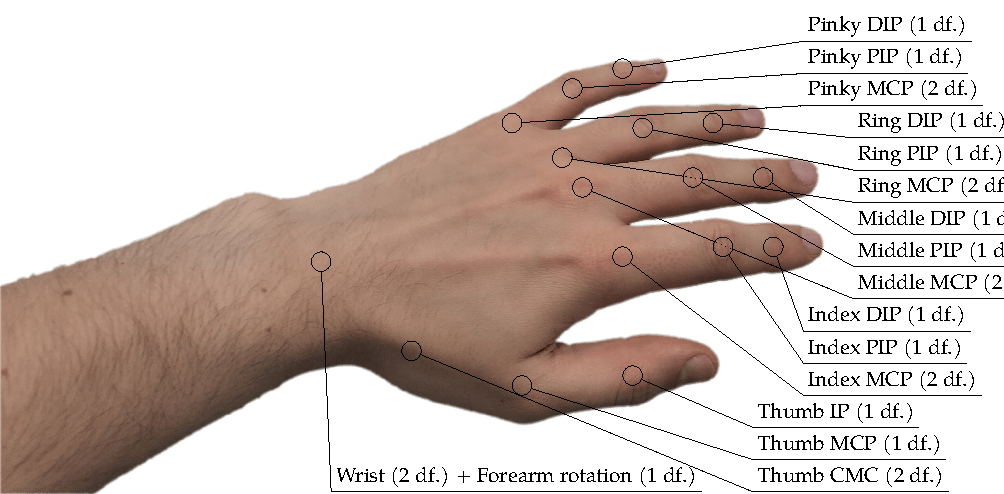
\includegraphics[width=1.1\linewidth]{figures/hand-joints.pdf}
    \captionsetup{parskip=7pt}
    \caption[Joints of the hand]{Each hand has 16 joints - three per digit, plus the wrist.

    The wrist and the first joint on each digit (the metacarpophalangeal (MCP) joints) can rotate on two axes, and so each have 2 degrees of freedom. The rest (the proximal- and distal-interphalangeal (PIP \& DIP) joints) can only rotate on one axis, and have 1.

    This naive counting gives 22 degrees of freedom. In addition, we usually consider rotation of the forearm (about the longitudinal axis) to be part of the hand, modeling it as a third degree of freedom of the wrist, which brings the total to 23 degrees of freedom.

    23 degrees of freedom is only a first approximation. A fully-realistic hand model needs to account for more minor degrees of freedom, such as movement of the metacarpal bones, rotation of the digits around the longitudinal axis, and movement of the skin and muscles. }
    \label{fig:hand-joints}
\end{figure}

It is not so straightforward to assign an angle to each of those 23 degrees of freedom. There are a variety of different parameterizations of the joints we might choose from, and additionally we have the option of placing constraints on the range of values that the angles can take. In this section we will discuss some of the most common parameterizations, and the pros and cons of each.

\clearpage

\subsection{Hierarchy of Rotations}

The most common parameterization of the hand is to use a hierarchy of rotations. Each joint is represented as a rotation (using one of the representations discussed in the previous section), along with an position offset, both relative to the previous joint. The magnitude of the offset typically remains fixed, because it represents the length of the bone. The wrist rotation is a rotation relative to the reference frame of the forearm (or the global reference frame, if only the hands are being modeled). The pinky MCP rotation is relative to the reference frame of the wrist, the PIP is relative to the MCP and so on. This means that rotating the wrist will change the position of all the joints in the hand, and rotating the MCP will change the position of all the joints below it, etc.

The benefit of this parameterization are that it matches the real kinematics of the hand -- rotating the wrist does in fact change the position of all the joints in the hand. For this reason this parameterization is used for the experiments in \Cref{C:hand-model}.

\subsection{Constraints}

Rather than representing each joint with a full rotation, we can place constraints on the range of values that the rotation can take. For example, the following constraints are used by \cite{hand-constraints}:
\begin{align}
\label{eqn:constraints}
\begin{aligned}
    0° ≤ \theta_{\text{MCP-F}} ≤ 90° \\
    -15° ≤ \theta_{\text{MCP-AA}} ≤ 15° \\
    0° ≤ \theta_{\text{PIP}} ≤ 110° \\
    0° ≤ \theta_{\text{DIP}} ≤ 90° \\
\end{aligned}
\end{align}

Whether or not to place constraints on the motion depends on the domain. For example, if we are modeling the hand for a virtual reality application, we might want to constrain the motion to be realistic. However, if we are training a neural network, then we cannot place non-differentiable constraints on the data, and it is more common to simply allow the network learn the constraints from the data.

\subsection{Point Cloud Representation}

For different tasks, different paramterizations might be appropriate. Take for example \textit{pose estimation}, where the task is to find the position and rotation of the joints from an image or video. In this case, a point cloud representation is often used, where each joint is represented by a point in 3D space. The benefit of this representation is that it is very easy to estimate from an image or video, and it is also easy to interpolate between two configurations. To then use this representation for animation, it is then converted into the hierarchical representation.


\section{Loss functions for learning angles}

\Cref{C:background} introduced some loss functions such as the Mean Squared Error (MSE) (\Cref{ss:mse}), which trains the model to output the posterior expectation $\mathbb{E}(y | x)$, and the Gaussian negative-log-likelihood which trains the model to output the posterior distribution $N(y | \mu, \sigma)$. This section will discuss some related loss functions that are used when data sits on a manifold, such as angles on the unit circle $S^1$, or rotations on $S^3$.
\subsection{Arc distance loss}
\label{ss:arc-dist}

The most obvious loss function that we might use when training a model to output angles is the arc distance between two angles. This is the distance between the two angles on the unit circle, and is given by
\begin{align}
\label{eqn:arc-dist}
\begin{aligned}
    \mathcal{L}_{\text{arc}}(y, \hat{y}) &= \cos^{-1}(\cos(y - \hat{y}))
\end{aligned}
\end{align}
A graph of this loss function is shown in \Cref{fig:loss-arc}. The loss is zero when the two angles are equal, and increases linearly as the angles move further apart. This loss function is not differentiable at $y = \hat{y} + \pi$, but this is not a problem because the model will never output this value.


\subsection{Angular mean squared error loss}
\label{ss:amse}

The analogous loss functions to the mean squared error for data that sits on the unit circle is the \textit{angular} mean-squared-error (eg. \cite{circ-statistics}), which will be used later on in \Cref{C:hand-model}. It is defined as follows:
\newcommand{\amse}{\mathcal{L}_{\theta\text{-MSE}}}
\begin{align}
\label{eqn:amse}
\begin{split}
    \fdef{\amse}{\R^{N×D}×\R^{N×D}}{\R} \\
    \amse&(Y, \hat{Y})_{ni} ≝ \frac{1}{N} \sum_{n, i} (\sin Y_{ni} - \sin \hat{Y}_{ni})^2 + (\cos Y_{ni} - \cos \hat{Y}_{ni})^2
\end{split}
\end{align}
where $Y$ and $\hat{Y}$ are sequences of vectors of angles, with batch shape $N$ and vector length $D$. We can see that the definition is similar to that of the circular mean in \Cref{ss:circ-mean}. A graph of the angular mean squared error loss is shown in \Cref{fig:loss-amse}.

\begin{figure}
    \centering
    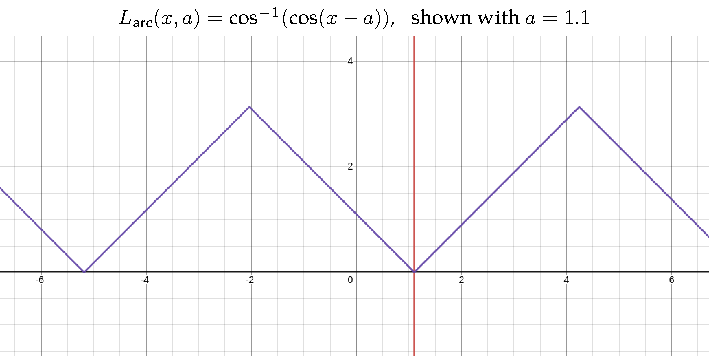
\includegraphics[width=0.9\linewidth]{figures/loss-arc.pdf}
    \captionsetup{parskip=7pt}
    \caption[Arc distance loss]{The arc distance loss function is the distance between two angles on the unit circle, analogous to the absolute distance for unbounded variables. It is zero when the two angles are equal, and increases linearly as the angles move further apart. The function is not differentiable at $y = \hat{y}$ and $y = \hat{y} + \pi$.}
    \hrulefill
    \label{fig:loss-arc}
\end{figure}
\begin{figure}
    \centering
    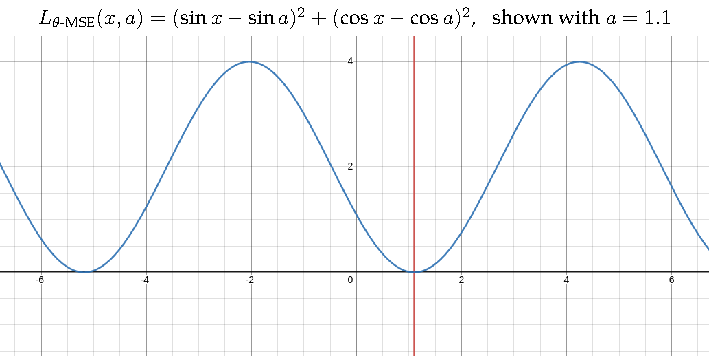
\includegraphics[width=0.9\linewidth]{figures/loss-amse.pdf}
    \captionsetup{parskip=7pt}
    \caption[Angular mean squared error loss]{The angular mean squared error loss function is analogous to the squared error for unbounded variables. It is zero when the two angles are equal, and increases quadratically as the angles move further apart, reaching a maximum when the two angles are opposite. Unlike the arc distance loss, the angular mean squared error loss is differentiable everywhere.}
    \label{fig:loss-amse}
\end{figure}

\clearpage


\subsection{Motivation for the Angular Mean Squared Error}
\label{ss:amse-motivation}

The angular mean squared error defined above in \Cref{ss:amse} is not arbitrarily chosen - it is the Maximum Likelihood Estimator (MLE) for the von-Mises distribution (the circular analogue of the Gaussian). The motivation and derivation for it is described in this subsection. First, for context, the derivation of the mean-squared-error from the likelihood function of the Gaussian distribution is given, and then the derivation of the angular mean-squared-error from the likelihood function of the von-Mises distribution.

As introduced in \Cref{ss:von-mises}, the von-Mises distribution is a distribution over angles on the unit circle. The Gaussian distribution and the von-Mises distribution are the \textit{maximum entropy} distributions of their respective domains. This means among all distributions over the real line $x \in (-\infty, \infty)$ with finite mean $\mu$ and variance $\sigma^2$, the Gaussian distribution $N(x \mid \mu, \sigma)$ is the one with the largest entropy. Similarly, among all distributions over the unit circle $x \in (-\pi, pi]$ with circular mean $\mu$ and circular variance $\kappa$, the von-Mises distribution is the one with the largest entropy.

As a result of this fact, training a model which outputs only a mean estimate with a mean-squared-error loss is equivalent to maximizing the likelihood of the data under the Gaussian distribution.

The likelihood function of a Gaussian distribution is as follows, where the mean $\mu$ is the output of the model $f(x, \theta)$.
\begin{align}
\label{notation:gaussian-likelihood}
\begin{aligned}
    \fdef{\mathbb{L}_G}{\R^P}{\R} \\
    \mathbb{L}_G&(\theta) ≝ \prod_n \frac{1}{\sqrt{2\pi\sigma^2}} \exp\left( -\frac{1}{2\sigma^2} (y_n - f(x_n, \theta))^2 \right)
\end{aligned}
\end{align}
where $x$ and $y$ are the input and target data respectively, $N$ is the number of data points, and $P$ is the number of parameters. For simplicity this is defined for scalar data, but the definition can be extended to vector data.

The optimization of the parameters $\theta$ is represented with the $\arg \max$ operator, which returns the value of $\theta$ that maximizes the likelihood of the data. Let $x$ and $y$ be the input and target data respectively, $N$ be the number of data points, and $P$ be the number of parameters.

The derivation is as follows:
\begin{align}
\label{eqn:gaussian-likelihood}
\begin{aligned}
    &\arg \max_\theta \mathbb{L}_G(\theta) \\
    = &\arg \max_\theta \prod_n \frac{1}{\sqrt{2\pi\sigma^2}} \exp\left( -\frac{1}{2\sigma^2} (y_n - f(x_n, \theta))^2 \right) \\
    = &\arg \max_\theta \prod_n \exp\left( -\frac{1}{2\sigma^2} (y_n - f(x_n, \theta))^2 \right) &&\text{by monotonicity} \\
    = &\arg \max_\theta \prod_n \exp\left( - (y_n - f(x_n, \theta))^2 \right) &&\text{by monotonicity} \\
    = &\arg \max_\theta \sum_n - (y_n - f(x_n, \theta))^2 &&\text{by monotonicity of} \ln \\
    = &\arg \min_\theta \sum_n (y_n - f(x_n, \theta))^2 \\
    = &\arg \min_\theta \frac{1}{N} \sum_n (y_n - f(x_n, \theta))^2 &&\text{by monotonicity} \\
    = &\arg \min_\theta \mse(y, f(x, \theta))
\end{aligned}
\end{align}

Similarly to the relationship between $\mse$ and the Gaussian, minimizing the angular mean-squared-error loss is equivalent to maximizing the likelihood of a von-Mises distribution. The likelihood function of a von-Mises distribution is as follows, where the circular mean $\mu$ is the output of the model $f(x, \theta)$.
\begin{align}
    \label{notation:von-mises-likelihood}
    \begin{aligned}
        \fdef{\mathbb{L}_\text{vM}}{\R^P}{\R} \\
        \mathbb{L}_\text{vM}&(\theta) ≝ \prod_n \frac{1}{2\pi I_0(\kappa)} \exp\left( \kappa \cos(y_n - f(x_n, \theta)) \right)
    \end{aligned}
\end{align}
where $x$ and $y$ are the input and target data respectively, $N$ is the number of data points, and $P$ is the number of parameters.
Again, for simplicity this is defined for scalar data, but the definition can be extended to vectors of angles.

Maximizing the above likelihood function is equivalent to minimizing the angular mean-squared-error loss. The derivation is as follows:
\begingroup
\allowdisplaybreaks
\begin{align*}
&\arg \max_{\theta} \mathbb{L}_\text{vM}(\theta) \\
= &\arg \max_{\theta} \prod_n \frac{1}{2\pi I_0(\kappa)} \exp\left( \kappa \cos(y_n - f(x_n, \theta)) \right) \\
= &\arg \max_{\theta} \prod_n \exp\left( \kappa \cos(y_n - f(x_n, \theta)) \right) &&\text{by monotonicity} \\
= &\arg \max_{\theta} \prod_n \exp\left( \cos(y_n - f(x_n, \theta)) \right) &&\text{by monotonicity} \\
= &\arg \max_{\theta} \sum_n \cos(y_n - f(x_n, \theta)) &&\text{by monotonicity of} \ln \\
= &\arg \min_{\theta} \sum_n - \cos(y_n - f(x_n, \theta)) \\
= &\arg \min_{\theta} \sum_n - \cos(y_n - f(x_n, \theta)) + 1 + 1 \\
= &\arg \min_{\theta} \sum_n - \cos(y_n - f(x_n, \theta)) + (\sin^2 y_n + \cos^2 y_n) \\
    &+ (\sin^2 f(x_n, \theta) + \cos^2 f(x_n, \theta)) &&\text{by} \sin^2 a + \cos^2 a = 1 \\
= &\arg \min_{\theta} \sum_n - (\sin y_n \sin f(x_n, \theta) + \cos y_n \cos f(x_n, \theta)) \\
    &+ (\sin^2 y_n + \cos^2 y_n) + (\sin^2 f(x_n, \theta) + \cos^2 f(x_n, \theta)) &&\begin{aligned}\text{by} &\cos(a ± b) \\ = &\cos a \cos b ∓ \sin a \sin b \end{aligned} \\
= &\arg \min_{\theta} \sum_n (\sin^2 y_n - \sin y_n \sin f(x_n, \theta) + \sin^2 f(x_n, \theta)) \\
    &+ (\cos^2 y_n - \cos y_n \cos f(x_n, \theta) +  \cos^2 f(x_n, \theta)) \\
= &\arg \min_{\theta} \sum_n (\sin^2 y_n + 2 \sin y_n \sin f(x_n, \theta) + \sin^2 f(x_n, \theta)) \\
    &+ (\cos^2 y_n + 2 \cos y_n \cos f(x_n, \theta) + 2 \cos^2 f(x_n, \theta)) &&\text{by monotonicity} \\
= &\arg \min_{\theta} \sum_n (\sin^2 y_n - 2 \sin y_n \sin f(x_n, \theta) + \sin^2 f(x_n, \theta)) \\
    &+ (\cos^2 y_n - 2 \cos y_n \cos f(x_n, \theta) + \cos^2 f(x_n, \theta)) \\
= &\arg \min_{\theta} \sum_n (\sin y_n - \sin f(x_n, \theta))^2 \\
    &+ (\cos y_n - \cos f(x_n, \theta))^2 \\
= &\arg \min_{\theta} \amse(y_n, \sin f(x_n, \theta)) \numberthis \label{eqn:amse-von-mises-derivation}
\end{align*}
\endgroup

\chapter{Hand Motion Model}
\label{C:hand-model}


I experimented with a variety of different model architectures,


% table of loss values
\begin{tabular}{ | c | c |}
    \hline
    Loss Value mean across whole dataset & 0.07275154 \\
    \hline
\end{tabular}


\section{Predicting the next frame}
\label{S:mean-model}


\section{Learning a probabilistic model}
\label{S:prob-model}

\chapter{Conclusions}
\label{C:conclusion}

To conclude, the main conclusions from the experiments in \Cref{C:a-o-sampling} and \Cref{C:hand-model}, are summarized, along with some reflections on the project as a whole.

\section{Conclusions}

\TODO{Add conclusions from the experiments.}

\section{Reflections}

If I had known what I know now at the start of my project, what would I have done differently?

First, training neural networks can be very finnicky. Instead of trying new architectures and model types, I later found that hyperparameters such as the weight initialization, learning rate, and regularization loss terms have a much bigger impact, including on whether the network learns anything reasonable at all. I would have spent more time tuning these hyperparameters, and less time tuning the number of layers, number of neurons, activation functions, and other architecture choices. Relatedly, during the middle of my project, I was working with a custom implementation of a transformer, which was learning poorly. If I was experimenting primarily with these different kinds of hyperparameters, I would have kept using the standard transformer implementation, which would have saved me significant implemenation and debugging time.

Second, training with Masked Sequence Modeling is sufficient to represent the task I was trying to achieve in Chapter 4, but I didn't know this at the outset. I could have used a mostly-pre-implemented data pre-processing pipeline, again saving me significant implementation and debugging time.

Third, running comparison experiments was forever a weak point for me. Doing this project again, I would have spent the additional effort to keep every version of my experiments working in the same codebase simultaneously, so that I could easily switch between them and compare results. Rather than modifying the implementation to run a new experiment (\textit{even if} the current model \& hyperparameters were currently broken), I would have added additional flags and configurations for every experiment, and added some unit tests to make sure that the code still works when these flags are changed.  This would have meant I could have produced more meaningful results in \Cref{C:hand-model}.

\section{Final words}

I have enjoyed working on this thesis, more than I expected at the outset. I have found a passion for learning about deep learning. The project has been challenging but has given me the opportunity to learn an immense amount about machine learning techniques, including modern methods such as transformers. Applying this knowledge to hand motion modeling has also been a challenge of surprising depth. I hope that this thesis has been a useful contribution to the field of hand motion modeling, and that it might be useful to others.



%%%%%%%%%%%%%%%%%%%%%%%%%%%%%%%%%%%%%%%%%%%%%%%%%%%%%%%

% and of course book style knows about backmatter
% \backmatter caused problems with appendices :-(
% and of course report style doesn't
%%%%%%%%%%%%%%%%%%%%%%%%%%%%%%%%%%%%%%%%%%%%%%%%%%%%%%%


%\bibliographystyle{ieeetr}
\printbibliography


\end{document}
